\chapter{Transformadas Integrales}

\section{Serie de Fourier}

\subsection{Periodicidad y paridad de funciones}

% \subsection{Funciones periódicas}

\begin{defi} \marginnote{Función periódica}
Una función $f: \mathbb{R} \to \mathbb{C} $ se dice que es \textbf{periódica de período} $T$, con $T\neq 0$, si 
\begin{equation} \label{Periodica}
    \boxed{
f(t) = f(t + T), \quad \forall \ t \in \mathbb{R}.}    
\end{equation}



La constante $T$ la tomaremos como la  menor constante positiva que satisface la igualdad \eqref{Periodica}.
\end{defi}


\begin{propiedad} 
    \textbf{Propiedades de las funciones periódicas.}
    \begin{enumerate}
        \item Si $f$ es periódica de periodo $T$, entonces $$f(t) = f(t + nT), \quad n = 0, \pm 1, \pm 2, \dots$$
        
        \item Si $f(t)$ y $g(t)$ son funciones periódicas de período $T$, entonces la función
        $$h(t) = \alpha f(t) + \beta g(t); \quad \alpha, \beta \in \mathbb{C},$$
        tiene el mismo período $T$.
    
        \item En general, si la función 
        $$f(t) = \cos (\omega_1 t) + \cos (\omega_2 t)$$
        es periódica de período $T$, entonces es posible encontrar dos enteros $n$ y $m$ tales que 
        \begin{align}
            \omega_1 T &= 2\pi n,  \label{Periodica1}\\
             \omega_2 T &= 2\pi m. \label{Periodica2}
        \end{align}
        
        El cociente de \eqref{Periodica1} y \eqref{Periodica2} es
        $$\frac{\omega_1}{\omega_2} = \frac{n}{m} \ ,$$
        es decir, la relación $\omega_1/ \omega_2$ debe ser un número racional.
    \end{enumerate}
\end{propiedad}


\begin{ejemplo}
Encuentre el período de la función $f(t) = \cos \left(\frac{t}{3}\right) + \cos \left(\frac{t}{4}\right)$.

\textbf{Solución:} Si la función $f(t)$ es periódica con período $T$, entonces, de \eqref{Periodica},
$$\cos \frac{1}{3}(t + T) + \cos \frac{1}{4}(t + T) = \cos \frac{t}{3} + \cos \frac{t}{4}.$$

Como $\cos(\theta + 2\pi n) = \cos \theta, n \in \mathbb{Z}$, obtenemos que 
$$\frac{1}{3} T = 2\pi n, \quad \frac{1}{4}T = 2\pi m; \quad n,m \in \mathbb{Z}.$$

Por consiguiente $T = 6\pi n = 8\pi m$; cuando $n = 4$ y $m=3$, se obtiene el mínimo valor de $T$. Así, $T = 24\pi$.
\end{ejemplo}

\begin{defi} \marginnote{Función seccionalmente continua}
    Una función $f: [a,b] \longrightarrow \mathbb{C}$ es \textbf{seccionalmente continua} si $[a,b]$ tiene una partición finita $a = t_0 < t_1 < \cdots < t_n = b$ tal que $f$ es continua y acotada en cada intervalo abierto $(t_i, t_{i+1}), i = 0, \dots, n-1$.
    
    Denotaremos por $\mathscr{C}[a,b]$ al conjunto de las funciones complejas seccionalmente continuas.
\end{defi}


\begin{propo}
Sea $f: \mathbb{R} \longrightarrow \mathbb{C}$ una función periódica de período $T$. Sea $a \in \mathbb{R}$, entonces
$$ \int_{a-T/2}^{a + T/2} f(t) \,dt = \int_{- T/2}^{T/2} f(t) \,dt .$$
\end{propo}

\begin{demo}
Utilizando la propiedad de aditividad de las integrales,
\begin{equation*}
    \int_{a-T/2}^{a + T/2} f(t) \,dt = \int_{a - T/2}^{-T/2} f(t) \,dt + \int_{- T/2}^{a + T/2} f(t) \,dt.
\end{equation*}

Haciendo la sustitución  $t = t' - T ~\Rightarrow~ dt = dt'$ en la primera integral, obtenemos
\begin{align*}
   \int_{a - T/2}^{-T/2}f(t) \,dt + \int_{- T/2}^{a + T/2} f(t) \,dt   &= \int_{a + T/2}^{T/2} f(t'-T) \,dt' + \int_{- T/2}^{a + T/2} f(t) \,dt \\
   &= \int_{a + T/2}^{T/2} f(t'-T + T) \,dt' + \int_{- T/2}^{a + T/2} f(t) \,dt \\
   &= \int_{a + T/2}^{T/2} f(t') \,dt' + \int_{-T/2}^{a + T/2} f(t) \,dt \\
   &= \int_{-T/2}^{T/2} f(t) \,dt.
\end{align*}
\end{demo}

\begin{defi}\marginnote{Extensión periódica}
Sea $f: [a,b] \rightarrow \mathbb{R}$ seccionalmente continua, se llama \textbf{extensión periódica} de $f$ a la función $f_e: \mathbb{R} \rightarrow \mathbb{R}$,
\begin{equation} 
    \boxed{f_e(t) = f(t + k_0 (b-a))} \ , 
\end{equation}
donde $k_0 \in \mathbb{Z}$ es el único entero que verifica $t + k_0(b-a) \in [a,b].$
\end{defi}

\begin{ejemplo}
La extensión periódica de $f \in \mathscr{C}[-\pi,\pi]$ real es
$$f_e(t) = f_e(t + 2\pi)$$

\begin{figure}[H]
    \centering
    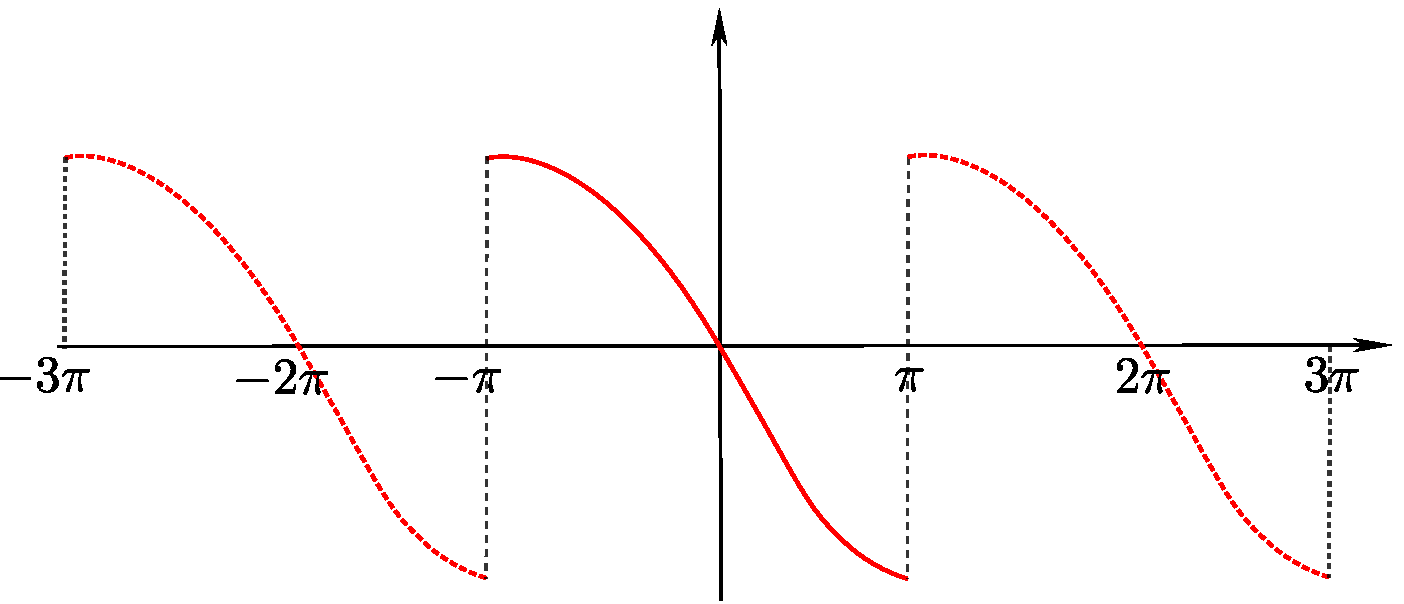
\includegraphics[scale = 0.45]{Figuras/Periocidad.pdf}
    \caption{Extensión periódica de una función real seccionalmente continua en $[-\pi,\pi]$.}
\end{figure}
\end{ejemplo}

% \subsection{Funciones pares e impares}
 
\begin{defi} \marginnote{Funciones pares e impares}
Sea $f: [-a,a] \longrightarrow \mathbb{R}$ perteneciente a $\mathscr{C}[-a,a]$.
Diremos que $f$ es una \textbf{función par} si y solo si, para todo $x$ en el intervalo $[-a,a]$, se cumple que
\begin{equation}
    f(-t) = f(t) \ .
\end{equation}
De forma similar, diremos que $f$ es una \textbf{función impar} si y solo si, para todo $x$ en el intervalo $[-a,a]$, se cumple que
\vspace{-0.1cm}
\begin{equation}
     f(-t) = -f(t) \ .
\end{equation}
\end{defi} 

\begin{propo}
    Sea $f: [-a,a] \longrightarrow \mathbb{R}$ integrable,
    \begin{align*}
        f ~\mbox{es par} &\Rightarrow \int_{-a}^a f(t) \,dt = 2 \int_0^a f(t) \,dt. \\
        f ~\mbox{es impar} &\Rightarrow \int_{-a}^a f(t) \,dt = 0.
    \end{align*}
\end{propo}

\begin{obs}{Observación}
    Toda función $f:[-a,a] \longrightarrow \mathbb{R}$ puede expresarse como la suma de una función par más otra impar: $f = f_p + f_i$ con 
    \begin{equation*}
        f_p(t) = \frac{f(t) + f(-t)}{2}, \quad f_i(t) = \frac{f(t) - f(-t)}{2} \ .
    \end{equation*}
\end{obs}

\begin{defi} \marginnote{Extensión par e impar}
Sea $f \in \mathscr{C}[0,a]$ real, entonces la \textbf{extensión par} y la \textbf{extensión impar} de $f$ están definidas, respectivamente, por:
\begin{equation*}
    E_f(t) = \left\{ \begin{array}{cll}
    f(-t)     & \mbox{si} & -a \leq t < 0 \\
    f(t)     & \mbox{si} & 0 \leq t \leq a
    \end{array} \right. , ~ O_f(t) = \left\{ \begin{array}{cll}
    -f(-t)     & \mbox{si} & -a \leq t < 0 \\
    f(t)     & \mbox{si} & 0 \leq t \leq a
    \end{array} \right. .
\end{equation*}
Ambas extensiones se encuentran definidas en el intervalo $[-a,a]$.
\end{defi}

\begin{figure}[H]
    \centering
    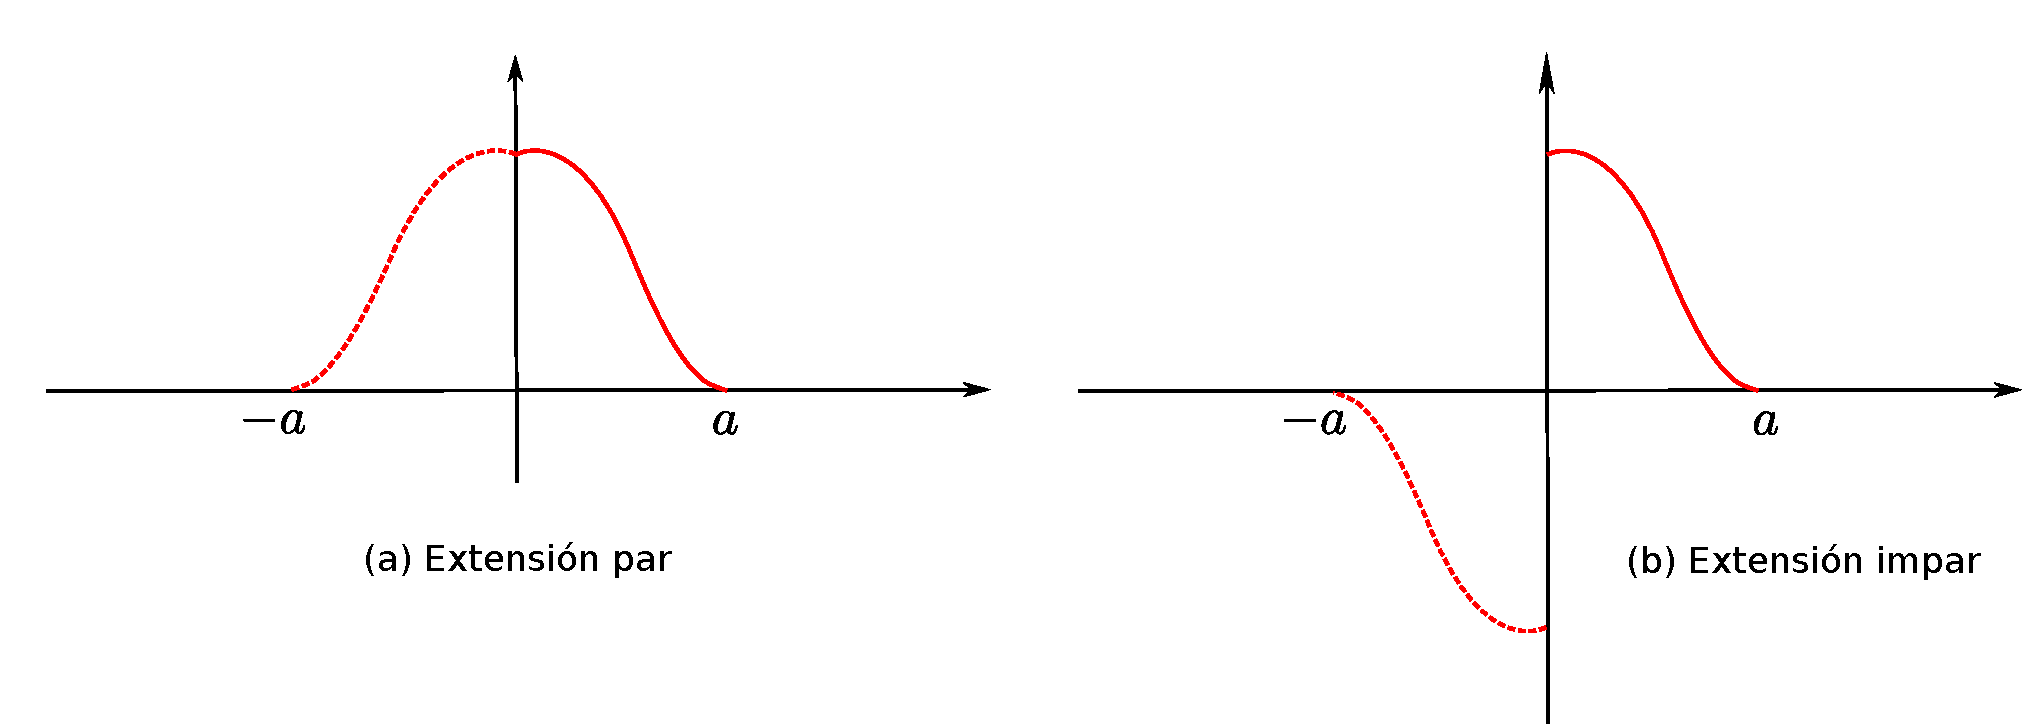
\includegraphics[width = \textwidth]{Figuras/Paridad.pdf}
    \caption{Extensión par e impar de una función real seccionalmente continua en $[0,a]$. }
\end{figure}

\subsection{Serie de Fourier trigonométrica}

% \subsection{Definición}

\begin{propo}
    En el espacio $\mathscr{C}[a,b]$, el conjunto formado por las funciones
    $$\left\{ 1, \cos\left( \frac{2n \pi}{T}x \right), \sin\left( \frac{2n \pi}{T}x \right) \right\}_{n=1}^{\infty}$$
    es un conjunto ortogonal, con $T = b-a$ el periodo de la función.
\end{propo}


\begin{defi} \marginnote{Sistema trigonométrico}
    Llamamos \textbf{sistema trigonométrico} al conjunto de funciones ortonormales en el espacio $\mathscr{C}[-\pi,\pi]$, definido como
    $$\left\{ \frac{1}{\sqrt{2\pi}}, \frac{\cos(nt)}{\sqrt{\pi}}, \frac{\sin(nt)}{\sqrt{\pi}} \right\}_{n=1}^{\infty}$$
\end{defi}

\begin{defi} \marginnote{Condiciones de Dirichlet}
    Una función $f$ satisface las llamadas \textbf{Condiciones de Dirichlet} si satisface
    \begin{enumerate}
        \item Se encuentra definida en un intervalo $(a,a+T)$.
        \item Tanto $f$ como su derivada son funciones seccionalmente continuas en el intervalo $(a,a+T)$.
        \item $f$ tiene un número finito de discontinuidades \emph{finitas}.
        \item $f$ es una función periódica de periodo $T$.
    \end{enumerate}

\end{defi}

\begin{defi} \marginnote{Serie de Fourier}
Sea $f \in \mathscr{C}[a, a+T]$ una función que satisface las condiciones de Dirichlet. Entonces, ella puede ser aproximada por la serie 
\begin{equation}
    \frac{a_0}{2} + \sum_{n=1}^{\infty} \left( a_n \cos\left( \frac{2n\pi}{T}x \right) + b_n \sin\left( \frac{2n\pi}{T}x \right) \right) \approx f(x) \ . \label{FourierTrigo}
\end{equation}

Esta expansión se denomina \textbf{serie trigonométrica de Fourier} o simplemente \textbf{serie de Fourier}, donde los \textit{coeficientes de Fourier} están dados por:
\begin{align*}
    a_0 &= \frac{2}{T} \int_{a}^{a+T} f(t) \,dt, \\
    a_n &= \frac{2}{T} \int_{a}^{a+T} f(t) \cos\left( \frac{2n\pi}{T}t \right) \,dt, \quad n = 1,2, \dots\\
    b_n &= \frac{2}{T} \int_{a}^{a+T} f(t) \sin\left( \frac{2n\pi}{T}t \right) \,dt. \quad n = 1,2, \dots
\end{align*}
\end{defi}

\begin{ejemplo} \label{EjemploFourier1}
    Consideremos la función $f(x) = x^2$ definida para $x\in [-\pi,\pi]$, la cual es continua con derivada $f'(x) = 2x$ también continua, luego la serie de Fourier de $f$ converge puntualmente a $f$ para todo $x \in (-\pi,\pi)$. Para los extremos $x = \pm \pi$ vemos que $f(\pi) = f(-\pi)$, por lo tanto la serie converge puntualmente a $f$ para todo $x \in [-\pi,\pi]$.
    
    Sus coeficientes de Fourier están dados por:
    \begin{align*}
        a_0 &= \frac{1}{\pi} \int_{-\pi}^{\pi} x^2 \,dx = \left. \frac{x^3}{3\pi} \right|_{-\pi}^{\pi} = \frac{2}{3} \pi^2, \\
        a_n &= \frac{1}{\pi} \int_{-\pi}^{\pi} x^2 \cos(n x)\,dx =   \left. \frac{1}{n\pi} x^2 \sin(nx)  \right|_{-\pi}^{\pi} - \frac{2}{n\pi} \int_{-\pi}^{\pi} x \sin(nx) \,dx\\
        &= \left.   \frac{2}{n^2\pi} x \cos(nx)\right|_{-\pi}^{\pi} - \frac{2}{n^2 \pi} \cancelto{0}{\int_{-\pi}^{\pi} \cos(nx) \,dx }\\
        &=  \frac{4}{n^2} \cos(n\pi) =  (-1)^n \frac{4}{n^2}, \quad n = 1,2,\dots\\
         b_n &= \frac{1}{\pi} \int_{-\pi}^{\pi} x^2 \sin(nx)\,dx = 0, \quad n = 1,2, \dots
    \end{align*}
    
    Entonces, su serie de Fourier es
    \begin{equation}
    f(x) = \frac{\pi^2}{3} + \sum_{n=1}^{\infty} (-1)^n \frac{4}{n^2} \cos(nx), \qquad x \in [-\pi,\pi].    \label{FourierCuadratica}
    \end{equation}
    
    Es claro que la serie de Fourier de $f(x) = x^2$ para todo $x\in \mathbb{R}$ representa la extensión periódica de los valores de $f(x)$ en el intervalo $[-\pi,\pi]$.
    
    La gráfica de $f$ en conjunto con diferentes sumas parciales de su serie de Fourier están representadas en la figura \ref{fig:EjemploFourier1}. 
    
    % \begin{figure}[htb]
        \centering
        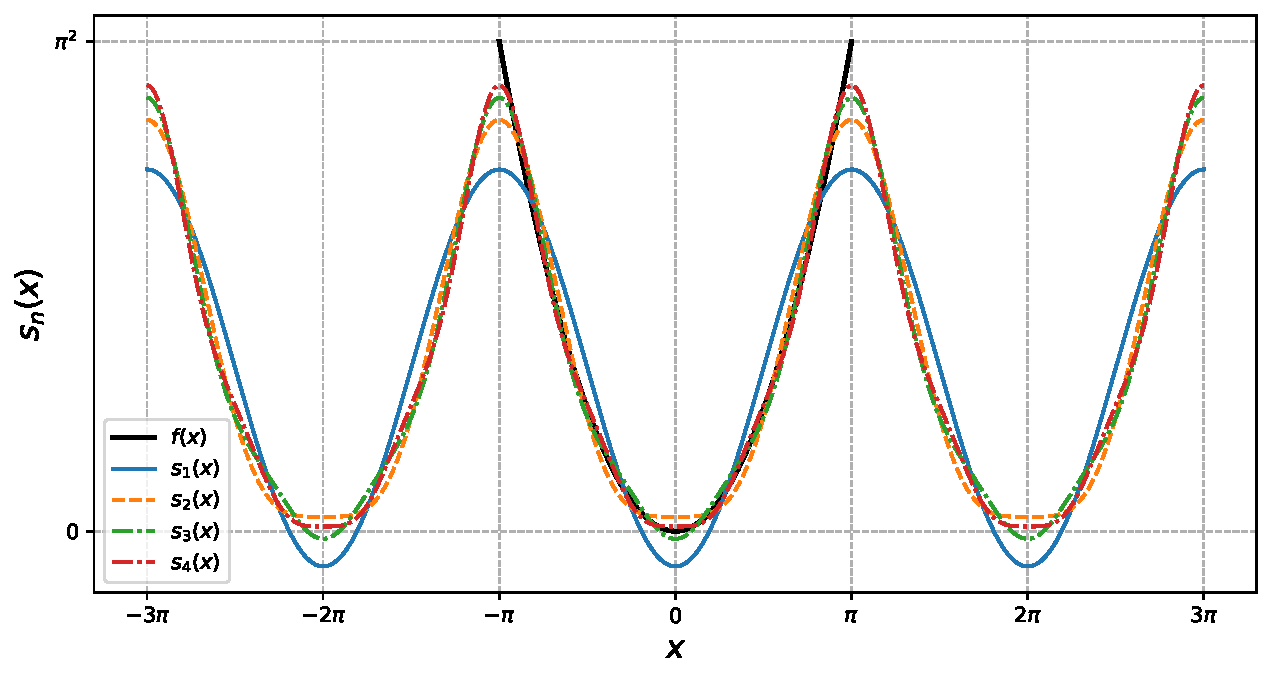
\includegraphics[width = 0.8\textwidth]{Figuras/EjemploFourier1.pdf}
        \captionof{figure}{Serie de Fourier de la función $f(x) = x^2, -\pi \leq x \leq \pi$, truncada hasta $n = 4$.}
        \label{fig:EjemploFourier1}
    % \end{figure}
    % El teorema visto para convergencia uniforme nos garantiza que esta serie converge uniformemente a $f(x) = x^2$ en $[-\pi,\pi]$, es más, al aplicar el criterio de M de Weierstrass a la serie, ésta converge para todo $x \in \mathbb{R}$, pues
    % $$\forall  x \in \mathbb{R}: ~ \left|(-1)^n \frac{4}{n^2} \cos(nx)\right| \leq \frac{4}{n^2} = M_n ~~\mbox{y}~~  \sum\limits_{n=1}^{\infty} M_n < \infty.$$
\end{ejemplo}

% \textbf{Observación}: La serie de Fourier de $f$ converge en media a $f$, o sea, 
% \begin{shaded}
% $$f(t) \sim \frac{a_0}{2} + \sum_{n=1}^{\infty} (a_n \cos(nt) + b_n \sin(nt)).$$    
% \end{shaded}

% \begin{propo} \label{C.FourierCero}
% Los coeficientes de la serie trigonométrica de Fourier de $f \in \mathscr{C}[-\pi,\pi]$ convergen a cero cuando $n \to \infty$, es decir,
% $$\lim_{n \to + \infty} a_n = \lim_{n \to + \infty} b_n = 0.$$
% \end{propo}

% \begin{demo}
% Si denotamos el sistema trigonométrico por 
% $$\varphi_0(t) = \frac{1}{\sqrt{2\pi}}, ~ \varphi_{2n-1}(t) = \frac{1}{\sqrt{\pi}} \cos(nt), ~ \varphi_{2n(t)} = \frac{1}{\sqrt{\pi}} \sin(nt), \quad n = 1,2, \dots$$

% tenemos que la serie generalizada de Fourier queda
% $$\sum_{n=0}^{\infty} C_n \varphi_n(t) = C_0 \varphi_0(t) + \sum_{n=1}^{\infty} \left[ C_{2n-1} \varphi_{2n-1}(t) + C_{2n} \varphi_{2n}(t) \right] ,$$

% la cual corresponde a la serie trigonométrica de Fourier de $f \in \mathscr{C}[-\pi,\pi]$, donde 
% $$a_0 = \sqrt{\frac{2}{\pi}} C_0, ~ a_n = \frac{C_{2n-1}}{\sqrt{\pi}}, ~ b_n = \frac{C_{2n}}{\sqrt{\pi}}, \quad n = 1,2, \dots$$

% De lo discutido en el primer capítulo, una de las consecuencias de la desigualdad de Bessel \eqref{D.Bessel} es que 
% $$\lim_{n \to + \infty} C_n = \lim_{n \to + \infty} \langle f, \varphi_n \rangle = 0 ~\Rightarrow~ \lim_{n \to \infty} C_{2n-1} = \lim_{n \to \infty} C_{2n} = 0. $$

% Por lo tanto, 
% $$\lim_{n \to + \infty} a_n = \lim_{n \to + \infty} b_n = 0.$$

% \end{demo}

% ¿Convergerá puntual y/o uniformemente la serie de Fourier a $f(t)$? ¿Qué condiciones deben cumplirse?

% Antes de responder estas preguntas, primero justifiquemos que es suficiente trabajar con funciones a valores reales, a pesar de que los siguientes teoremas también son válidos para funciones a valores complejos. 

\subsubsection{Serie de Fourier de una función compleja de variable real}

Sea $f = u + iv \in \mathscr{C}[a,b]$, su serie de Fourier trigonométrica está dada por \eqref{FourierTrigo} con 
\begin{align*}
    a_0 &= \frac{2}{T} \int_{a}^{b} f(t) \,dt =  \frac{2}{T} \int_a^b u(t) \,dt + i\frac{2}{T} \int_a^b v(t) \,dt,\\
    a_n &= \frac{2}{T} \int_a^b f(t) \cos\left( \frac{2n\pi}{T}t \right) \,dt = \frac{2}{T} \int_a^b u(t) \cos\left( \frac{2n\pi}{T}t \right) \,dt + i\frac{2}{T} \int_a^b v(t) \cos\left( \frac{2n\pi}{T}t \right) \,dt , \quad n \in \mathbb{N} \\
    b_n &= \frac{2}{T} \int_a^b f(t) \sin\left( \frac{2n\pi}{T}t \right) \,dt = \frac{2}{T} \int_a^b u(t) \sin\left( \frac{2n\pi}{T}t \right) \,dt + i\frac{2}{T} \int_a^b v(t) \sin\left( \frac{2n\pi}{T}t \right) \,dt, \quad n \in \mathbb{N}
\end{align*}

Entonces, su serie de Fourier nos queda
\begin{align}
  f(t) & \sim   \left\{ \frac{\real(a_0)}{2} + \sum_{n=1}^{\infty} \left[ \real(a_n) \cos\left( \frac{2n\pi}{T}t \right) + \real\left( b_n \right) \sin\left( \frac{2n\pi}{T}t \right) \right] \right\}  \nonumber \\
   & \qquad + i \left\{ \frac{\im(a_0)}{2} + \sum_{n=1}^{\infty} \left[\im(a_n) \cos\left( \frac{2n\pi}{T}t \right) + \im(b_n) \sin\left( \frac{2n\pi}{T}t \right) \right] \right\},
\end{align}

es decir, la serie de Fourier de $f = u + iv$ será dada por
\begin{equation}
    S_F(f) = S_F(u) + i S_F(v) \ ,
\end{equation}
donde $S_F$ representa a una serie de Fourier.


\subsection{Series de senos y cosenos}

\begin{defi} \marginnote{Serie de Fourier seno y serie de Fourier coseno}
    Dadas las extensiones par e impar de una función, $E_f, O_f: [a,b] \to \mathbb{R}$, es posible obtener el desarrollo en serie de Fourier de cada una de estas, que corresponden a los \textbf{desarrollos en serie de Fourier de coseno y de seno} de $f$, respectivamente. Estos son definidos como
    \begin{align*}
        E_f(t) & \sim \frac{a_0}{2}  + \sum_{n=1}^{\infty} a_n \cos\left( \frac{2n\pi}{T}t \right), & ~~\mbox{donde}~~ a_n = \frac{2}{T} \int_a^{b} f(t) \cos\left( \frac{2n\pi}{T}t \right)  dt \ , \\
        O_f(t) & \sim  \sum_{n=1}^{\infty} b_n \sin\left( \frac{2n\pi}{T}t \right), & ~~\mbox{donde} ~~ b_n = \frac{2}{T} \int_a^{b} f(t) \sin\left( \frac{2n\pi}{T}t \right) \ dt \ .
    \end{align*}

    En ambos casos, se ha hecho uso de las propiedades de las funciones pares e impares para hallar los coeficientes de las series.
\end{defi}

% Puesto que $E_f, O_f: [-\pi,\pi] \to \mathbb{R}$ son seccionalmente continuas, se puede obtener el desarrollo en serie de Fourier de estas, los cuales están definidos por: \footnote{La forma de las series seno y coseno, con sus respectivos coeficientes, se obtienen al aplicar las propiedades vistas para las funciones pares e impares.}
% $$ 

% y
% $$ .$$

% Estos son llamados \textbf{desarrollos en serie de Fourier de coseno y de seno de $f$}, respectivamente.

% \subsection{Convergencia puntual y uniforme}

% \begin{defi}
% Sea $f: [a,b] \longrightarrow \mathbb{R}$, para $t_0 \in [a,b]$ definimos
% \begin{align*}
%     f(t_0^+) &= \lim_{t \to t_0^+} f(t), \\
%     f(t_0^-) &= \lim_{t \to t_0^-} f(t),
% \end{align*}

% si existen los límites. 

% Una discontinuidad en $t_0$ tal que $f(t_0^+)$ y $f(t_0^-)$ existen se denomina \textbf{discontinuidad de salto} y $f(t_0^+) - f(t_0^-)$ recibe el nombre de \textbf{salto} de $f$ en $t_0$.
% \end{defi}

% \textbf{Observaciones:} 

% \begin{enumerate}
%     \item La magnitud del salto es $|f(t_0^+) - f(t_0^-)|$.
    
%     \item El salto se anula cuando $f(t_0) = f(t_0^+) = f(t_0^-)$, es decir, cuando $f$ es continua en $t_0$.
    
%     \item Una función $f: [a,b] \longrightarrow \mathbb{R}$ seccionalmente continua tiene discontinuidades de salto.
% \end{enumerate}

% \begin{defi}
% Sea $f:[a,b] \longrightarrow \mathbb{R}$, con una discontinuidad de salto en $t_0 \in [a,b]$, definimos la \textbf{derivada por la derecha} como 
% $$f'(t_0^+) = \lim_{h \to 0^+} \frac{f(t_0 + h ) - f(t_0^+)}{h}$$

% cuando el límite existe. Similarmente, definimos la \textbf{derivada por la izquierda} como 
% $$f'(t_0^-) = \lim_{h \to 0^-} \frac{f(t_0 + h ) - f(t_0^-)}{h}$$

% cuando el límite existe.
% \end{defi}

% \begin{teorema}[Convergencia puntual de la serie de Fourier] \label{Puntual}
% Sea $f(t)$ una función real seccionalmente continua en el intervalo $-\pi < t < \pi$. Su serie de Fourier trigonométrica converge al valor medio
% \vspace{-0.05cm}
% $$\frac{f(t^+) + f(t^-)}{2}$$

% para cada $t \in (-\pi,\pi)$ donde ambas derivadas laterales $f'(t^+)$ y $f'(t^-)$ existen.
% \end{teorema}

% \textbf{Observación:} Si denotamos por $f_e$ a la extensión periódica de $f$, a partir del teorema anterior, la expansión en serie de Fourier converge a $f_e$ para todo $x \in \mathbb{R}$ al extenderla periódicamente al valor medio
% $$\frac{f_e(t^+) + f_e(t^-)}{2}.$$

% De hecho, en los extremos $t = \pm \pi$, la serie converge a 
% $$\frac{f(-\pi^+) + f(\pi^-)}{2}.$$

% En efecto, observemos que
% $$f_e(-\pi^+) = f(-\pi^+) ~~\mbox{y}~~ f_e(-\pi^-) = f(\pi^-).$$

% Luego, el cociente
% $$\frac{f_e(-\pi^+) + f_e(-\pi^-)}{2} = \frac{f(-\pi^+) + f(\pi-)}{2}.$$

% Análogamente para $t = \pi$.

% \begin{teorema}[Convergencia uniforme] \label{C.Uniforme}
% Supóngase que $f$ es continua en $[-\pi,\pi]$, $f(-\pi) = f(\pi)$ y que $f'$ es continua por tramos, con discontinuidades de salto. Entonces la serie de Fourier trigonométrica de $f$ converge a $f$ absolutamente y uniformemente.
% \end{teorema}

% \subsection{Ejemplos}



% Podemos usar la expansión en serie de Fourier de $f(x) = x^2$ en $[-\pi,\pi]$ para probar que 
% $$\sum_{n=1}^{\infty} \frac{1}{n^2} = 1 + \frac{1}{4} + \frac{1}{9} + \cdots = \frac{\pi^2}{6}.$$

% En efecto, al evaluar $x = \pi$ en \eqref{FourierCuadratica}, obtenemos que 
% $$f(\pi) = \frac{\pi^2}{3} + \sum_{n=1}^{\infty} (-1)^n \frac{4}{n^2} \cos(n\pi) = \frac{\pi^2}{3} + \sum_{n=1}^{\infty} (-1)^{2n} \frac{4}{n^2} = \frac{\pi^2}{3} +  \sum_{n=1}^{\infty} \frac{4}{n^2}.$$

% Así,
% $$\pi^2 = \frac{\pi^2}{3} + 4 \sum_{n=1}^{\infty} \frac{1}{n^2} \Rightarrow \sum_{n=1}^{\infty} \frac{1}{n^2} = \frac{\pi^2}{6}.$$

\begin{ejemplo} \label{Signo}
Consideremos la función signo  definida por
$$f(x) := \left\{ \begin{array}{cc}
     -1,& - \pi \leq x < 0  \\
     1,&   0 \leq x \leq \pi
\end{array} \right. .$$

La función es seccionalmente continua con $x = 0$ punto de discontinuidad de salto y las derivadas laterales existen para todo $x \in (-\pi,\pi)$, luego la serie de Fourier de $f$ converge puntualmente a $f$ en los puntos de continuidad y a 
$$\frac{f(0^-) + f(0^+)}{2} = 0, \quad \mbox{en} ~ x = 0 ~~\mbox{y}$$
$$\frac{f(-\pi^+) + f(\pi^-)}{2} = 0, \quad \mbox{en} ~ x = \pm \pi. $$

Sus coeficientes de Fourier están dados por:
\begin{align*}
    a_0 &= \frac{1}{\pi} \int_{-\pi}^{\pi} f(x) \,dx = 0 , \\
    a_n &= \frac{1}{\pi} \int_{-\pi}^{\pi} f(x) \cos(n x)\,dx = 0, \quad n = 1,2,\dots
\end{align*}
\begin{align*}
     b_n &= \frac{1}{\pi} \int_{-\pi}^{\pi} f(x) \sin(nx) \,dx \\
     &= \frac{1}{\pi} \int_{-\pi}^0 (-1) \sin(nx)\,dx + \frac{1}{\pi} \int_{0}^{\pi} (1) \sin(nx) \,dx \\
     &= \left.  \frac{1}{\pi n} \cos(nx) \right|_{-\pi}^0 - \left. \frac{1}{\pi n} \cos(nx) \right|_{0}^{\pi} \\
     &= \frac{2}{\pi n} [1 - (-1)^n] \\
     &= \left\{ \begin{array}{cl}
         0, & n ~\mbox{par}  \\
         \frac{4}{\pi n}, &  n ~\mbox{impar}
     \end{array} \right. .
\end{align*}

Entonces, su serie de Fourier es 
$$f(x) =  \sum_{n ~impar} \frac{4}{\pi n} \sin(nx) = \sum_{k=1}^{\infty} \frac{4}{\pi} \frac{\sin[(2k-1)x]}{ (2k-1)}.$$

\textbf{Aclaración:} Note que a pesar de haber escrito que la función $f$ es igual a la serie, debemos tener en cuenta que en los punto $x = 0$ y $x = \pm \pi$ converge al valor medio del salto de la discontinuidad.

Es claro que la serie de Fourier de $f$ para todo $x\in \mathbb{R}$ representa la extensión periódica de los valores de $f(x)$ en el intervalo $[-\pi,\pi]$.

La gráfica de $f$ en conjunto con diferentes sumas parciales de su serie de Fourier están representadas en la figura \ref{fig:EjemploFourier2}.

\begin{figure}[H]
    \centering
    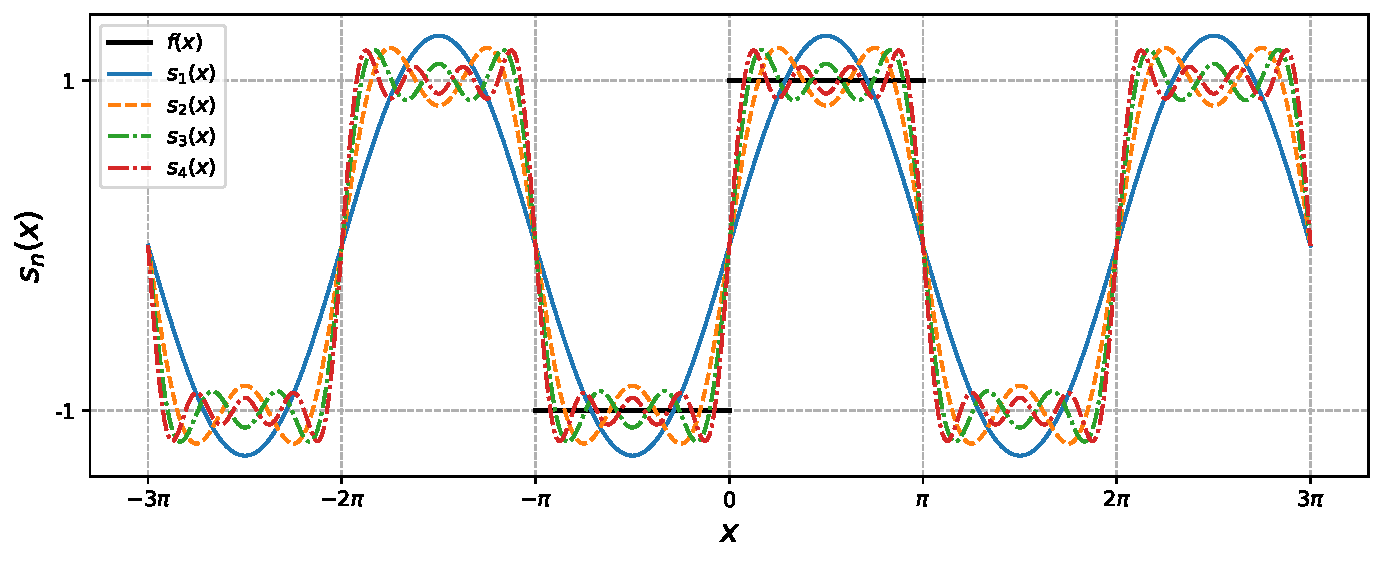
\includegraphics[scale = 0.65]{Figuras/EjemploFourier2.pdf}
    \caption{Serie de Fourier de la función signo truncada hasta $n = 4$.}
     \label{fig:EjemploFourier2}
\end{figure}

\end{ejemplo}

\subsection{Serie exponencial}

\begin{propo}
    En el espacio $\mathscr{C}[a,a+T]$, el conjunto formado por las funciones 
    \begin{equation}
        \left\{ \frac{1}{\sqrt{T}} \exp\left(i\frac{2n\pi}{T}x\right) \right\}_{n= - \infty}^{n = \infty}
    \end{equation}
    es un conjunto ortonormal.
\end{propo}

\begin{defi} \marginnote{Sistema exponencial}
    Llamamos \textbf{sistema exponencial} al conjunto de funciones ortonormales en el espacio $\mathscr{C}[-\pi,\pi]$, definido como 
    $$\left\{ \frac{1}{\sqrt{2\pi}} e^{int} \right\}_{n= - \infty}^{n = \infty}$$
\end{defi}

\begin{defi} \marginnote{Serie de Fourier exponencial}
Sea $f \in \mathscr{C}[a,a+T]$ una función con un número finito de discontinuidades. Entonces, ella puede ser aproximada por la serie 
\begin{equation}
     \sum_{n=- \infty}^{\infty} c_n \exp\left(i\frac{2n\pi}{T}x\right) \label{FourierExpo}
\end{equation}

Esta expansión se denomina \textbf{serie exponencial de Fourier}  donde los \textit{coeficientes de Fourier} están dados por:
\begin{equation*}
    c_n = \frac{1}{T} \int_{a}^{a+T} f(t) \exp\left(-i\frac{2n\pi}{T}t \right) \ dt \ .
\end{equation*}
\end{defi}

% \textbf{Observación}: La serie de Fourier de $f$ converge en media a $f$, o sea, 
% \begin{shaded}
%  $$f(t) \sim \sum_{n=- \infty}^{\infty} c_n e^{int}.$$   
% \end{shaded}

\begin{propo} \label{TrigoExpo}
La $n$-ésima suma parcial de la serie de Fourier trigonométrica de una función (real o compleja) es igual a la $n$-ésima suma parcial de la serie exponencial.
\end{propo}

\begin{demo}
La $n$-ésima suma parcial de la serie exponencial es
$$ s_n(t) = \sum_{k=-n}^n c_k e^{ikt}.$$

Separando la suma:
\begin{align*}
    s_n(t) &= \sum_{k=-n}^{-1} c_k e^{ikt} + c_0 + \sum_{k=1}^n c_k e^{ikt} \\
    &= c_0 + \sum_{k=1}^n c_k e^{ikt} + \sum_{k=1}^n c_{-k} e^{-ikt} \\
    &= c_0 + \sum_{k=1}^n [c_k e^{ikt} + c_{-k} e^{-ikt}]. 
\end{align*}

Usando la identidad de Euler, $e^{i\theta} = \cos(\theta) + i \sin(\theta)$, encontramos que
$$s_n(t) = c_0 +  \sum_{k=1}^n [(c_k + c_{-k}) \cos(kt) + i(c_k - c_{-k}) \sin(kt)].$$

Desarrollando los coeficientes de la serie exponencial de Fourier, tenemos que
\begingroup
\allowdisplaybreaks
\begin{align*}
    c_0 &= \frac{1}{2\pi} \int_{-\pi}^{\pi} f(t) \,dt, \\
    c_k + c_{-k} &= \frac{1}{2\pi} \int_{-\pi}^{\pi} f(t) e^{-ikt} \,dt + \frac{1}{2\pi} \int_{-\pi}^{\pi} f(t) e^{ikt} \,dt  \\
    &= \frac{1}{2\pi} \int_{-\pi}^{\pi} f(t) [e^{ikt} + e^{-ikt}] \,dt \\
    &= \frac{1}{\pi} \int_{-\pi}^{\pi} f(t) \cos(kt) \,dt; \quad k = 1,2, \dots\\
   i( c_k - c_{-k}) &= \frac{i}{2\pi} \int_{-\pi}^{\pi} f(t) e^{-ikt} \,dt - \frac{i}{2\pi} \int_{-\pi}^{\pi} f(t) e^{ikt} \,dt \\
   &= - \frac{i}{2\pi} \int_{-\pi}^{\pi} f(t) [e^{ikt} - e^{-ikt}] \,dt \\
   &= \frac{1}{\pi} \int_{-\pi}^{\pi} f(t) \sin(kt)\,dt; \quad k = 1,2, \dots
\end{align*}
\endgroup

Comparando las expresiones obtenidas con los coeficientes de la serie de Fourier trigonométrica, podemos concluir que 
$$c_0 = \frac{a_0}{2}, ~  c_k + c_{-k} = a_k, ~ i( c_k - c_{-k}) = b_k; \quad k = 1,2, \dots$$

Por lo tanto, 
$$ s_n(t) = \sum_{k=-n}^n c_k e^{ikt} = \frac{a_0}{2} + \sum_{k=1}^n (a_k \cos(kt) + b_k \sin(kt)).$$

\end{demo}
Una consecuencia inmediata de la proposición \ref{TrigoExpo} es que todos los teoremas vistos para la serie de Fourier trigonométrica son aplicables a la serie de Fourier exponencial.

\begin{propiedad} 
    \textbf{Propiedades de la Serie de Fourier exponencial}
    \begin{enumerate}
        \item Los coeficientes de las series \eqref{FourierTrigo} y \eqref{FourierExpo} están relacionados por 
        \begin{equation}
        a_0 = 2c_0,~~ a_n = c_n + c_{-n}, ~~ b_n = i(c_n - c_{-n}); \quad n = 1,2, \dots    \label{RelacionCoefi1}
        \end{equation}
        
        o bien, 
        \begin{equation}
            c_n = \left\{ \begin{array}{cl}
                \frac{1}{2} (a_n - ib_n), & n \geq 0  \\
            \frac{1}{2}(a_{-n} + i b_{-n}),     & n  \leq -1 
            \end{array} \right. . \label{RelacionCoefi2}
        \end{equation}

        \item Si $f(t)$ es una función real, entonces sus respectivos coeficientes complejos $c_n$ satisfacen la relación:
        $$c_n^* = \frac{1}{2\pi} \int_{-\pi}^{\pi} f(t) (e^{-int})^* \,dt = \frac{1}{2\pi} \int_{-\pi}^{\pi} f(t) e^{int} \,dt = c_{-n}\ .$$
    \end{enumerate}
\end{propiedad}




\section{Transformada de Fourier}

En el capítulo anterior, aprendimos que la serie de Fourier de $f \in \mathscr{C}[-L/2,L/2]$ está dada por 
\begin{equation} \label{Transformada1}
  f(x) = \sum_{n=-\infty}^{\infty} c_n e^{i \frac{2n\pi}{L}x} \ ,  
\end{equation}
donde 
\begin{equation} \label{Transformada2}
  c_n = \frac{1}{L} \int_{-L/2}^{L/2} f(x) e^{-i\frac{2n\pi}{L}x} \,dx, \quad n \in \mathbb{Z} \ . 
\end{equation}

Una consecuencia inmediata de la expansión en serie de Fourier es que la función $f(x)$ representada por la serie resulta periódica, con período $L$. Por lo tanto, decimos que la serie de Fourier permite \emph{expandir funciones periódicas}. 

Sin embargo, no todas las funciones son periódicas, y nos interesará expandirlas dentro de algún intervalo de validez. Necesitamos, entonces, algún modo de expandir, en una base ortonormal, funciones no periódicas. 

Podemos decir que el conjunto de coeficientes $\{c_n\}$ también definen a $f(x)$. Este conjunto de números $c_n$ puede ser entendido como una función en la variable $n$, escrita como $c(n)$, definida para un conjunto \emph{discreto} de valores de la variable independiente (en lugar de un intervalo continuo).  
\begin{defi}\marginnote{Espectro de Fourier}
    Se define como el \textbf{espectro de Fourier} a la función de variable discreta $c(n)$, definida a partir de los coeficientes de Fourier \eqref{Transformada2}.
\end{defi}

El espectro de una función puede ser graficado, asumiendo $c(n)$ real, como se observa en la figura \ref{fig:espectro-fourier}.

\vspace{-0.5cm}
\begin{figure}[H]
    \centering
    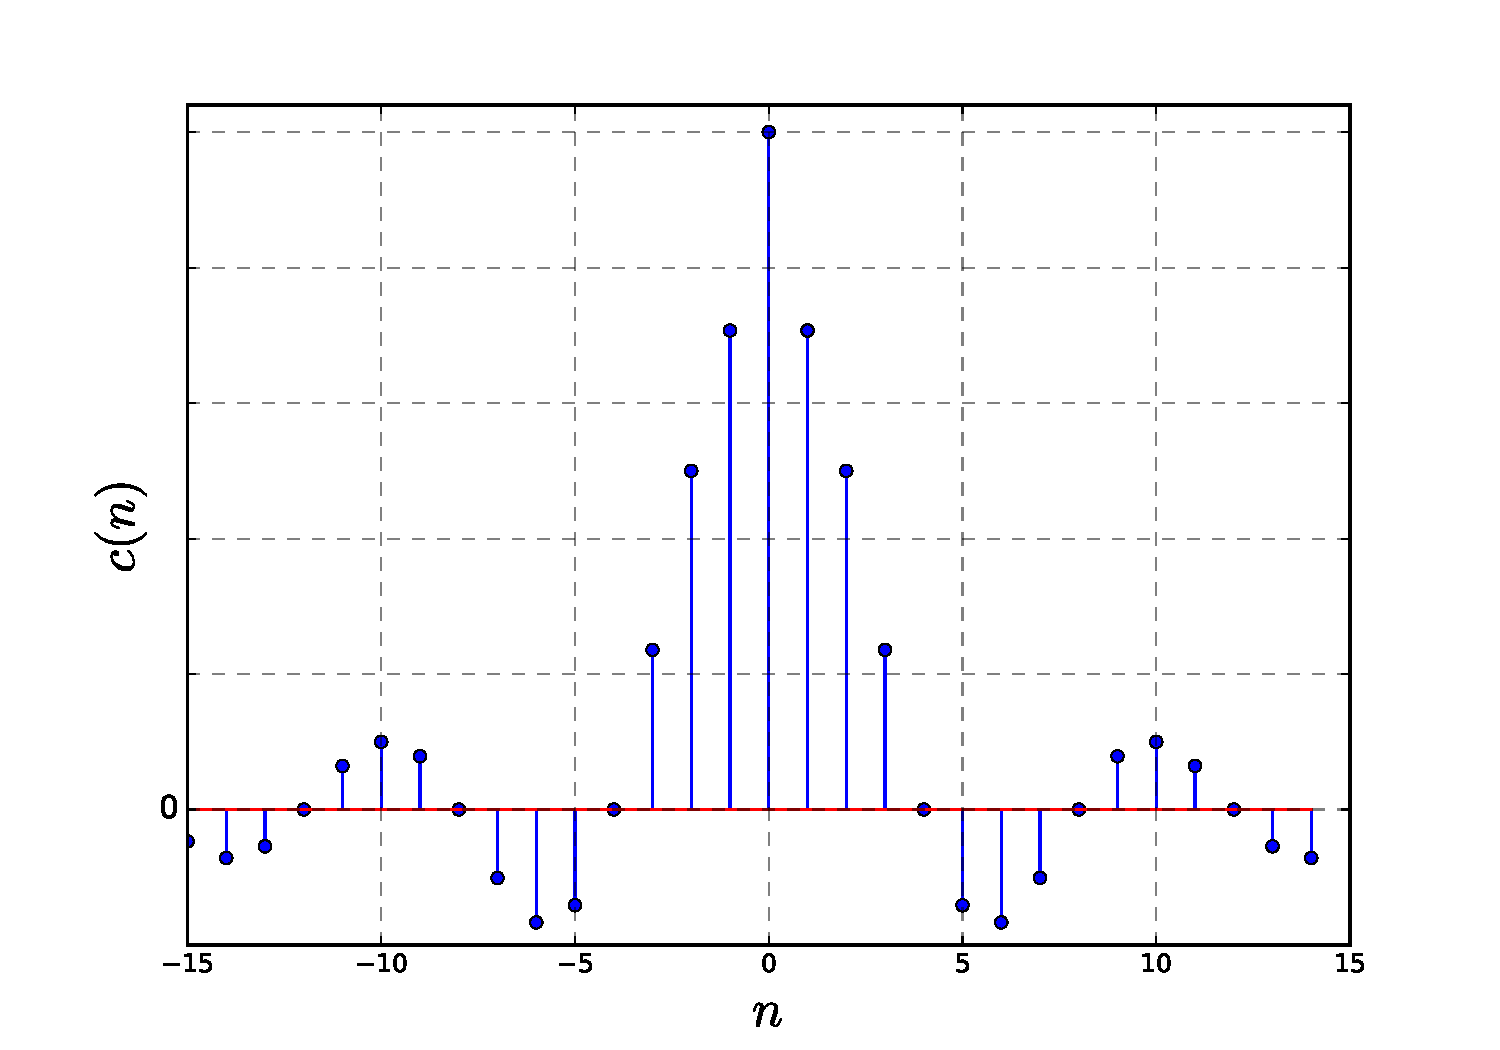
\includegraphics[width = 12cm]{Figuras/Espectro1.pdf}
    \caption{Espectro de Fourier.}
    \label{fig:espectro-fourier}
\end{figure}

En lugar de graficar $c$ vs $n$, podemos graficar $c$ vs $k$, el \emph{número de onda}, que corresponde a la frecuencia asociada a la parte espacial:
$$k = \frac{2\pi n}{L}.$$

Si $L \to \infty$, entonces las frecuencias se encuentran estrechamente espaciadas debido a que la diferencia entre valores consecutivos de $k$ es
$$\Delta k = \frac{ 2\pi \Delta n}{L}  = \frac{2\pi}{L}, \quad \mbox{pues}~ \Delta n = 1.$$

En otras palabras, para $L \to \infty$, $\Delta k$ es pequeño. Con este cambio de escala, el espectro de Fourier puede parecerse a lo mostrado en la figura \ref{Espectro1}.

\begin{figure}
    \centering
    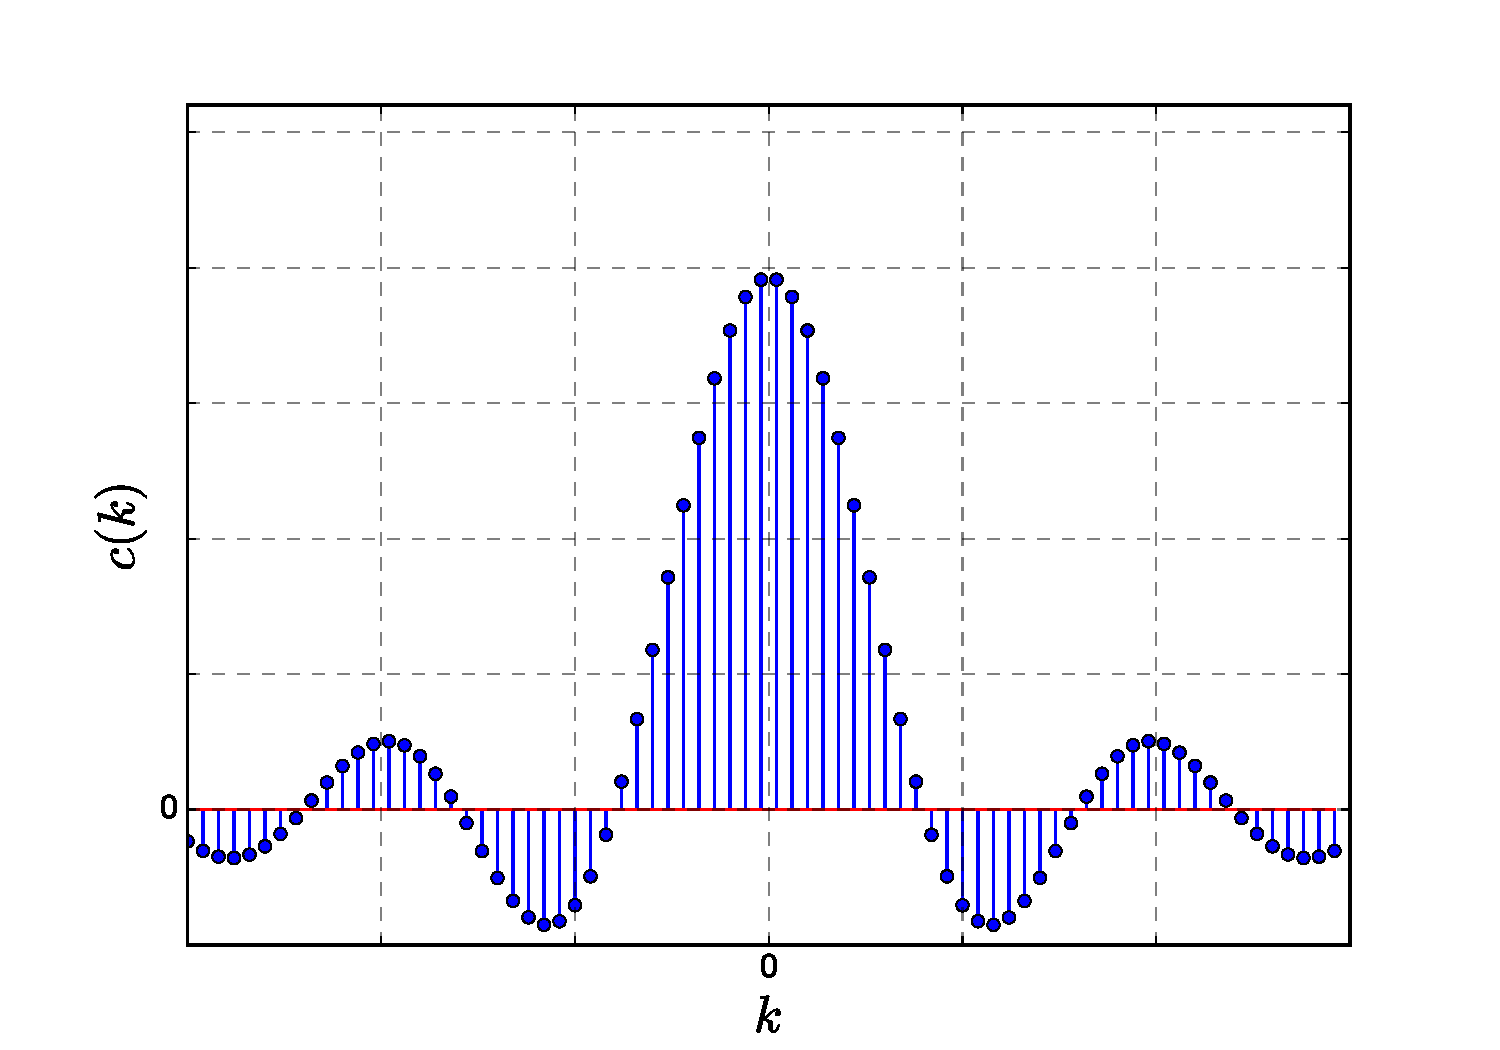
\includegraphics[scale = 0.4]{Figuras/Espectro2.pdf}
    \caption{Espectro de Fourier cuando $L \to + \infty$.}
    \label{Espectro1}
\end{figure}

Es natural especular sobre la posibilidad de un espectro continuo cuando $L$ tiende al infinito  de tal forma que todas las frecuencias están presentes. Puede ser instructivo considerar la siguiente derivación heurística: Sabemos que una función puede ser expandida como una serie de Fourier tal como se muestra en \eqref{Transformada1}. Luego, la transición $L \to \infty$ puede resultar difícil de realizar directamente ya que $c_n$ aparentemente tiende a cero. Seguimos entonces la idea de usar las frecuencias $k = 2\pi n/L$ tal que
$\Delta k = (2\pi/L ) \Delta n = 2\pi/L$ para valores de $k$ adyacentes y definimos
\begin{equation}
    c_L(k) = \frac{L}{\sqrt{2 \pi}} c_n \ .
\end{equation}

Usando las definiciones anteriores en las ecuaciones \eqref{Transformada1} y \eqref{Transformada2}, obtenemos que la función y sus coeficientes de Fourier se pueden escribir como: 
\begin{align*}
    f(x)&= \sum_{Lk/2\pi = -\infty}^{\infty} \frac{\sqrt{2\pi}}{L} c_L(k) e^{ikx} \left( \frac{\Delta k L}{2\pi}\right) = \sum_{Lk/2\pi = -\infty}^{\infty}  \frac{1}{\sqrt{2\pi}} c_L(k) e^{ikx} \Delta k , \\
  c_L(k) &= \frac{L}{\sqrt{2\pi}} \frac{1}{L} \int_{-L/2}^{L/2} f(x) e^{-ikx} dx = \frac{1}{\sqrt{2\pi}} \int_{-L/2}^{L/2} f(x) e^{-ikx} dx.
\end{align*}

Al hacer $L \to \infty$, la función $f$ puede considerarse como una función no-periódica arbitraria definida en todo el intervalo $(-\infty, \infty)$, mientras que la primera suma ``se convierte'' en una integral:
\begin{align*}
    f(x)& = \frac{1}{\sqrt{2\pi}} \int_{-\infty}^{\infty} c(k) e^{ikx} \,dk, \\
  c(k) & = \lim_{L\to + \infty} c_L(k) = \frac{1}{\sqrt{2\pi}} \int_{-\infty}^{\infty} f(x) e^{-ikx} dx.
\end{align*}

\begin{defi} \marginnote{Transformada de Fourier}
    Dada una función $f$ no periódica definida en $\mathscr{C}(-\infty, \infty)$, definimos su \textbf{transformada de Fourier} como 
    \begin{equation}\label{T.Fourier}
        \boxed{\tilde{f}(k) := \frac{1}{\sqrt{2\pi}} \int_{-\infty}^{\infty} f(x) e^{-ikx} dx \ .} 
    \end{equation}  
\end{defi}

Note que la transformada de Fourier es la extensión natural del concepto de series de Fourier para funciones no periódicas. Además, al ser $n$ una variable discreta, y $k$ continua, podemos decir que la transformada de Fourier es la generalización del concepto de series de Fourier cuando las funciones pertenecen a un espacio vectorial de dimensión continua.

\begin{defi}\marginnote{Transformada inversa de Fourier}
    Se define la \textbf{transformada inversa de Fourier} como
      \begin{equation}\label{I.Fourier}
     \boxed{f(x) = \frac{1}{\sqrt{2\pi}} \int_{-\infty}^{\infty} \tilde{f}(k) e^{ikx} \,dk \ .} 
    \end{equation}  
\end{defi}

\begin{obs}{Observaciones}
    \begin{itemize}
        \item Otras notaciones usadas son: $\tilde{f}(k) = \hat{f}(k) = g(k) = \mathcal{F}\{f(x)\}(k)$.
        
        \item El factor $1/\sqrt{2\pi}$ en la definición \eqref{T.Fourier} es convencional. Lo importante es que se cumpla la identidad conocida como \textbf{integral de Fourier}
        \begin{equation}
            f(x) = \int_{-\infty}^{\infty} \left[\frac{1}{2\pi} \int_{-\infty}^{\infty} f(\xi) e^{-ik\xi} d\xi \right] e^{ikx} \,dk.
          \label{IntegralFourier}
        \end{equation}
       
        % Por ejemplo, en lugar de estos factores, podría introducirse un $\alpha$ en \eqref{I.Fourier} y $1/(2\pi \alpha)$ en \eqref{T.Fourier}, con $\alpha$ una constante arbitraria. Algunas elecciones populares son: $\alpha = 1$ y $\alpha = 1/\sqrt{2\pi}$ \cite{Rubilar}.
    
        \item Al igual que el factor $1/\sqrt{2\pi}$ en la definición \eqref{T.Fourier}, la función $e^{-ikx}$ es convencional y puede ser reemplazada por $e^{ikx}$, siempre y cuando se verifique \eqref{IntegralFourier} \cite{Butkov, Riley}.
        
        % \item En el caso que $f(x)$ sea real, tenemos que \eqref{IntegralFourier} se puede escribir como 
        % \begin{equation}
        %     f(x) = \frac{1}{\pi} \int_{0}^{\infty} \int_{-\infty}^{\infty} f(\xi) \cos k(x-\xi)  \, d\xi \,dk.  \label{IntegralFourierReal}
        % \end{equation}
    
        % \colorlet{shadecolor}{blue!10} 
        % \begin{shaded}
        % En efecto, la relación \eqref{IntegralFourier} también se puede expresar como 
        % $$f(x) = \frac{1}{2\pi}  \int_{-\infty}^{\infty} \int_{-\infty}^{\infty} f(\xi) e^{-ik\xi} e^{ikx} d\xi  \,dk = \frac{1}{2\pi}  \int_{-\infty}^{\infty} \int_{-\infty}^{\infty} f(\xi) e^{ik(x-\xi)} d\xi  \,dk.$$
        
        % Como $f(x)$ es real, se igualan las partes reales para así obtener
        % $$f(x) = \frac{1}{2\pi} \int_{-\infty}^{\infty} \int_{-\infty}^{\infty} f(\xi) \cos k(x-\xi) d\xi  \,dk. $$
        
        % Puesto que $\cos k(x-\xi)$ es par con respecto a $k$, tenemos que 
        % $$f(x) = \frac{2}{2\pi} \int_{0}^{\infty} \int_{-\infty}^{\infty} f(\xi) \cos k(x-\xi)  \, d\xi \,dk =\frac{1}{\pi} \int_{0}^{\infty} \int_{-\infty}^{\infty} f(\xi) \cos k(x-\xi)  \, d\xi \,dk. $$  
        % \end{shaded}
        % \colorlet{shadecolor}{green!20}
        
        \item Es común en Física trabajar con funciones del tiempo, $f = f(t)$. En este caso, se acostumbra usar la frecuencia $\omega$ en lugar del número de onda $k$, de modo que la transformada de Fourier adopta la forma
        $$
        f(t) = \frac{1}{\sqrt{2\pi}} \int_{- \infty}^{\infty} \Tilde{f}(\omega) e^{i \omega t} d\omega,
        $$
    
        donde
        $$
        \Tilde{f}(\omega) = \frac{1}{\sqrt{2\pi}} \int_{- \infty}^{\infty} f(t) e^{- i \omega t} dt.
        $$
        
        \item En 3 dimensiones, la integral de Fourier está dada por:
        \begin{align*}
             f(\vec{r}\,) &:= \frac{1}{(2\pi)^{3/2}} \int_{\mathbb{R}^3} \tilde{f}(\vec{k}) e^{i (\vec{k} \cdot \vec{r})} d^3k, \\
             \tilde{f}(\vec{k}\,) &:= \frac{1}{(2\pi)^{3/2}} \int_{\mathbb{R}^3} f(\vec{r}) e^{-i (\vec{k} \cdot \vec{r})} d^3x.
        \end{align*}
        
        En general, en $n$ dimensiones:
         \begin{align*}
             f(\vec{r}\,) &:= \frac{1}{(2\pi)^{n/2}} \int_{\mathbb{R}^n} \tilde{f}(\vec{k}) e^{i (\vec{k} \cdot \vec{r})} d^n k, \\
             \tilde{f}(\vec{k}\,) &:= \frac{1}{(2\pi)^{n/2}} \int_{\mathbb{R}^n} f(\vec{r}) e^{-i (\vec{k} \cdot \vec{r})} d^n x.
        \end{align*}
       
    \end{itemize}    
\end{obs}


% \textbf{Observaciones:}

¿Cómo aseguramos la existencia de la transformada de Fourier de una función? Para ello, necesitamos introducir el concepto de \emph{funciones absolutamente integrables}, tras lo cual podemos plantear el teorema de existencia de la transformada de Fourier.

\begin{defi} \marginnote{Función absolutamente integrable}
Si $f(x)$ es tal que 
$$\int_{-\infty}^{\infty} |f(x)| \,dx < \infty,$$

entonces se dice que $f \in  L^1$ o que es \textbf{absolutamente integrable}.
\end{defi}

\begin{teorema}
Si $f \in L^1$, entonces la transformada de Fourier $\tilde{f}(k) = \mathcal{F}\{f(x)\}(k)$ existe y $\lim\limits_{k \to \pm \infty} \tilde{f}(k) = 0$.
\end{teorema}

\begin{demo}

Demostraremos solo la primera parte del teorema.

Notemos que
$$e^{-ikx} = \cos(kx) - i \sin(kx) ~\Rightarrow~ |e^{-ikx}| = 1.$$

Luego,
$$ \int_{-\infty}^{\infty} |f(x) e^{-ikx}| dx =  \int_{- \infty}^{\infty} |f(x)| \,dx < \infty.$$

En consecuencia, $f(x) e^{-ikx}$ es absolutamente integrable y
$$\frac{1}{2\pi} \int_{-\infty}^{\infty} f(x) e^{-ikx} dx$$

es finita, es decir, $\tilde{f}(k)$ existe. 
\end{demo}

\begin{obs}{Observación}
    La condición de que $f$ sea absolutamente integrable es suficiente pero no necesaria para la existencia de la transformada de Fourier.
\end{obs}

\begin{teorema}
    Sea $f(x)$ una función seccionalmente continua en cada intervalo finito del eje $x$, y supongamos que es absolutamente integrable en $(-\infty, + \infty)$. Entonces la \textbf{integral de Fourier} satisface
\begin{equation}
    \frac{1}{\pi} \int_0^{+\infty} \int_{-\infty}^{+\infty} f(\xi) \cos k(\xi-x) \,d\xi dk = \frac{f(x^+) + f(x^-)}{2} \ ,    
\end{equation}
donde ambas derivadas laterales, $f'(x^+)$ y $f'(x^-)$, existen.
\end{teorema}

\begin{demo}
Consulte el cápitulo 6 <<Fourier Integrals and Applications>> en \cite{Brown}.
\end{demo}

% \section{Ejemplos}

\begin{ejemplo} \label{PulsoCuadrado}
    \textbf{Función pulso cuadrado.} Consideremos la función 
    \begin{equation*}
        f(x) = \left\{ \begin{array}{cl}
            1,& |x|<a  \\
            0,& |x|> a
        \end{array} \right. \ .
    \end{equation*}

    Su transformada de Fourier es 
    \begin{align}
        \tilde{f}(k) & = \frac{1}{\sqrt{2\pi}} \int_{-\infty}^{\infty} f(x) e^{-ikx} dx \nonumber \\
        & = \frac{1}{\sqrt{2\pi}}\int_{-a}^a (1)  e^{-ikx} dx \nonumber \\
        & = \frac{1}{\sqrt{2\pi}} \left[ - \frac{1}{ik} e^{-ikx} \right]_{-a}^a \nonumber\\
        & = \frac{1}{\sqrt{2\pi} i k} [e^{ika} - e^{-ika}] \nonumber\\
        & = \sqrt{\frac{2}{\pi}} \frac{\sin(ka)}{k} \ . \label{TransPulsoCuadrado}
    \end{align}

    \begin{figure}[H]
        \centering
        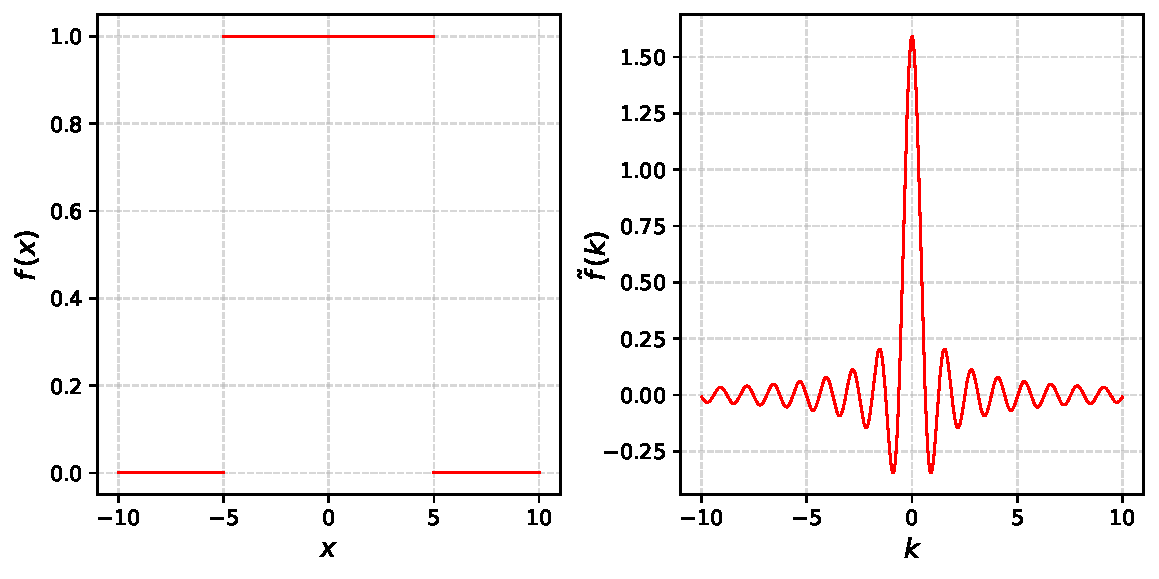
\includegraphics[scale = 0.55]{Figuras/EjemploTransformada1.pdf}
        \caption{Pulso cuadrado y su transformada de Fourier, con $a = 5$.}
        \label{Espectro2}
    \end{figure}

\end{ejemplo}

\begin{ejemplo}
    \textbf{Distribución gaussiana.} Considere la gaussiana
    \begin{equation*}
        f(x) = n e^{-\beta x^2}, \quad  \beta > 0 \ .
    \end{equation*}
    Su transformada de Fourier está dada por 
    \begin{equation*}
        \tilde{f}(k) =  \frac{n}{\sqrt{2\pi}} \int_{-\infty}^{\infty} e^{-\beta x^2} e^{-ikx} dx =  \frac{n}{\sqrt{2\pi}} \int_{-\infty}^{\infty} e^{-\beta x^2-ikx} dx .
    \end{equation*}

    Notemos que 
    \begin{align*}
        -\beta x^2-ikx &= - \beta \left( x^2 + \frac{ik}{\beta}x \right) \\
        &= - \beta \left( x^2 + \frac{ik}{\beta} x + \left( \frac{ik}{2\beta} \right)^2 - \left( \frac{ik}{2\beta} \right)^2 \right) \\
        &= - \beta \left( x + \frac{ik}{2\beta} \right)^2 + \beta \left( \frac{ik}{2\beta} \right)^2 \\
        &= - \beta \left( x + \frac{ik}{2\beta} \right)^2 - \left( \frac{k^2}{4\beta} \right).
    \end{align*}

    Luego, su transformada de Fourier puede escribirse como
    \begin{equation*}
        \tilde{f}(k) =  \frac{n}{\sqrt{2\pi}} \int_{-\infty}^{\infty} e^{-\beta \left( x + ik/2\beta \right)^2 - \left(k^2/4\beta \right)}  dx = \frac{n}{\sqrt{2\pi}} e^{- \left( k^2/4\beta \right)} \int_{-\infty}^{\infty} e^{-\beta \left( x + ik/2\beta \right)^2} \,dx. 
    \end{equation*}

    Haciendo el cambio de variable $u = x + \frac{ik}{2\beta}$, obtenemos que \footnote{}
    \begin{equation}\label{eq:Fourier-Gaussiana}
        \hat{f}(k) = \frac{n}{\sqrt{2\pi}} e^{- \left( k^2/4\beta \right)} \int_{-\infty}^{\infty} e^{-\beta u^2} \, du = \frac{n}{\sqrt{2\beta}} e^{- \left( k^2/4\beta \right)} \ ,
    \end{equation}
    donde hemos usado que 
    \begin{equation}
    \int_{-\infty}^{\infty} e^{-\beta x^2} \,dx = \sqrt{\frac{\pi}{\beta}}, \quad \beta > 0 \ . 
    \end{equation} 

    \begin{figure}[H]
        \centering
        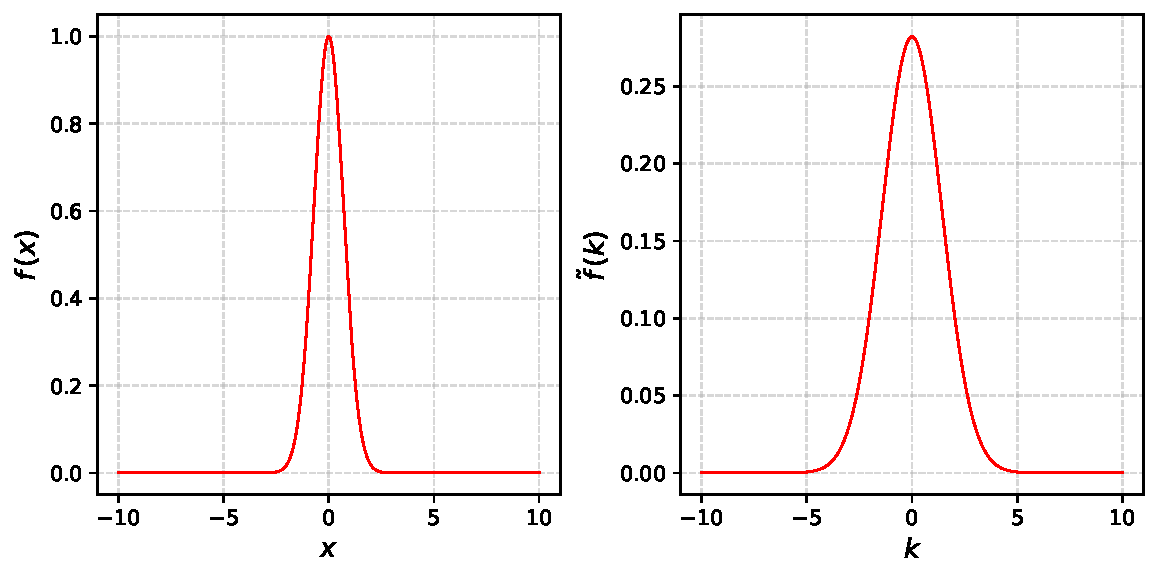
\includegraphics[width = 0.8\textwidth]{Figuras/EjemploTransformada2.pdf}
        \caption{Distribución gaussiana y su transformada de Fourier para $n=1$ y $\beta =1$ .}
        \label{Espectro3}
    \end{figure}
        \footnoterule
        
        {\footnotesize
        $^2$ En estricto rigor se debería calcular una integral compleja, vea \cite{Arfken}.
        }



    \begin{figure}[H]
        \centering
        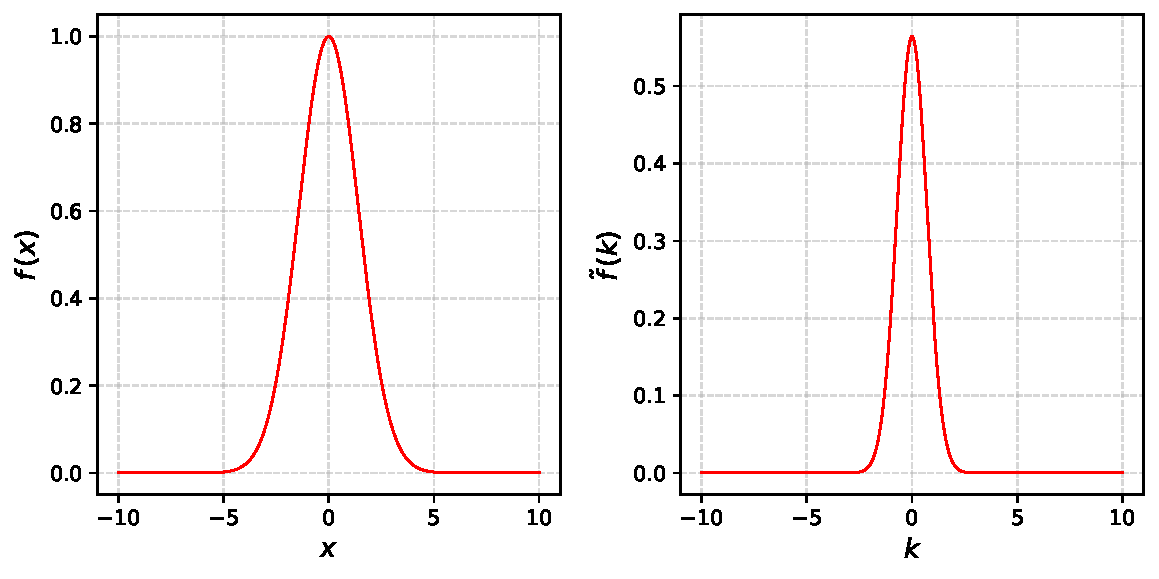
\includegraphics[scale = 0.6]{Figuras/EjemploTransformada3.pdf}
        \caption{Distribución gaussiana y su transformada de Fourier para $n=1$ y $\beta =0.25$ .}
        \label{Espectro4}
    \end{figure}
\end{ejemplo}


\subsection{Propiedades de la transformada de Fourier}

\begin{propiedad} 
\textbf{Propiedades de la Transformada de Fourier.} Sean las funciones $f, g \in L^1$ y los escalares $\alpha, \beta \in \mathbb{C}$.

\begin{enumerate}
    \item \textbf{Linealidad}: $$\mathcal{F}\{\alpha f(x) + \beta g(x)\}(k) = \alpha \mathcal{F}\{f(x)\}(k) + \beta \mathcal{F}\{g(x)\}(k).$$ 
    
    \item Si $f$ es real, entonces 
    % $$\tilde{f}(-k) = \tilde{f}^\ast(k).$$
    $$ \mathcal{F}\{f(x)\}(-k) = (\mathcal{F}\{f(x)\}(k))^*.$$
    
    \item \textbf{Traslación}: $$\mathcal{F}\{f(x+a)\}(k) = e^{ika} \mathcal{F}\{f(x)\}(k), \quad a \in \mathbb{R}.$$
    
    \item \textbf{Cambio de escala:} $$\mathcal{F}\{f(\alpha x)\}(k) = \frac{1}{|\alpha|}\mathcal{F}\{f(x)\}\left(\frac{k}{ \alpha}\right), \quad\alpha \neq 0.$$
    
    \item  \textbf{Atenuación}: $$\mathcal{F}\{f(x)e^{-ax}\}(k) =  \mathcal{F}\{f(x)\}(k-ia), \quad a \in \mathbb{C}.$$
    
    \item Si $f$ es una función par, entonces $\tilde{f}$ es una función real.
    
    \item Si $f$ es una función impar, entonces $\tilde{f}$ es una función puramente imaginaria, es decir, $\tilde{f}(k) = - \tilde{f}(-k)$.

    % \item \textbf{Escalonamiento:} $$\mathcal{F}\{f(\alpha x)\}(k) = \frac{1}{|\alpha|}\mathcal{F}\{f(x)\}\left(\frac{k}{ \alpha}\right), \quad\alpha \neq 0.$$
\end{enumerate}
\end{propiedad}

\begin{demo}
Demostraremos los puntos desde el 1 hasta el 5, y volveremos más tarde a los puntos 6 y 7.

\begin{enumerate}
    \item Por la definición \eqref{T.Fourier} de la transformada de Fourier y usando el hecho de que las funciones son absolutamente convergentes, tenemos
    \begin{align*}
        \mathcal{F}\{\alpha f(x) + \beta g(x)\}(k) &= \frac{1}{\sqrt{2\pi}} \int_{-\infty}^{\infty} [\alpha f(x) + \beta g(x)] e^{-ikx} dx \\
        &= \frac{\alpha}{\sqrt{2\pi}} \int_{-\infty}^{\infty}  f(x) e^{-ikx} dx + \frac{\beta}{\sqrt{2\pi}} \int_{-\infty}^{\infty}  g(x) e^{-ikx} dx \\
        &= \alpha \mathcal{F}\{f(x)\}(k) + \beta \mathcal{F}\{g(x)\}(k).
    \end{align*}
    
    \item Por la definición \eqref{T.Fourier} de la transformada de Fourier y suponiendo que $f$ es real:
    \begin{align*}
        \mathcal{F}\{f(x)\}(-k) &= \frac{1}{\sqrt{2\pi}} \int_{-\infty}^{\infty}  f(x)  e^{-(-ikx)} dx  \\
        &= \frac{1}{\sqrt{2\pi}} \int_{-\infty}^{\infty}  f(x)  (e^{-ikx})^* dx  \\
        &= \frac{1}{\sqrt{2\pi}} \int_{-\infty}^{\infty}  [f(x)  e^{-ikx}]^* dx \\
        &= (\mathcal{F}\{f(x)\}(k))^*.
    \end{align*}

    \item Por la definición \eqref{T.Fourier} de la transformada de Fourier, se tiene que
    \begin{equation*}
        \mathcal{F}\{f(x+a)\}(k) = \frac{1}{\sqrt{2\pi}}\int_{-\infty}^\infty f(x+a) e^{-ikx} dx \ .
    \end{equation*}

    Al hacer la sustitución $s = x+a$, $ds = dx$, tenemos
    \begin{align*}
        \frac{1}{\sqrt{2\pi}} \int_{-\infty}^\infty f(x+a)e^{-ikx}dx & = \frac{1}{\sqrt{2\pi}} \int_{-\infty}^\infty f(s) e^{-ik(s-a)} ds \\
        & = \frac{1}{\sqrt{2\pi}} \int_{-\infty}^\infty f(s) e^{-iks+ika} ds \\
        & = e^{ika} \left(\frac{1}{\sqrt{2\pi}} \int_{-\infty}^\infty e^{-iks} ds \right) \\
        & = e^{ika} \mathcal{F}\{f(x)\} (k) \ .
    \end{align*}

    \item Por la definición \eqref{T.Fourier} de la transformada de Fourier, se tiene que
    \begin{equation*}
        \mathcal{F} \{ f(\alpha x) \}(k) = \frac{1}{\sqrt{2\pi}} \int_{-\infty}^\infty f(\alpha x)e^{-ikx} dx \ .
    \end{equation*}

    Supondremos $\alpha > 0$. Haciendo el cambio de variable $u = \alpha x$, $du = \alpha dx$, tenemos
    \begin{equation*}
        \frac{1}{\sqrt{2\pi}} \int_{-\infty}^\infty f(\alpha x) e^{-ikx} dx = \frac{1}{\alpha} \left(\frac{1}{\sqrt{2\pi}} \int_{-\infty}^\infty f(u) e^{-i(k/\alpha)u} du \right) = \frac{1}{\alpha} \mathcal{F}\{f(x)\} \left( \frac{k}{\alpha} \right) \ .
    \end{equation*}

    Ahora, si $\alpha < 0$, hacemos el mismo cambio de variable que antes, obteniendo
    \begin{align*}
        \frac{1}{\sqrt{2\pi}} \int_{-\infty}^\infty f(\alpha x)e^{-ikx} dx & = \frac{1}{\alpha} \left( \frac{1}{\sqrt{2\pi}} \int_{\infty}^{-\infty} f(u) e^{-i(k/\alpha)u} du \right) \\ 
        & = - \frac{1}{\alpha} \left(\frac{1}{\sqrt{2\pi}} \int_{-\infty}^\infty f(u) e^{-i(k/\alpha)u} du \right) \\
        & = - \frac{1}{\alpha} \mathcal{F}\{f(x)\} \left(\frac{k}{\alpha}\right) \ .
    \end{align*}

    Por lo tanto, concluimos que, para $\alpha \neq 0$, se tendrá que
    \begin{equation*}
        \mathcal{F}\{(\alpha x)\}(k) = \frac{1}{|\alpha|} \mathcal{F}\{f(x)\} \left( \frac{k}{\alpha} \right) \ .
    \end{equation*}

    \item Por la definición \eqref{T.Fourier} de la transformada de Fourier, se tiene que
    \begin{align*}
        \mathcal{F}\{ f(x)e^{-ax} \}(k) & = \frac{1}{\sqrt{2\pi}} \int_{-\infty}^\infty f(x) e^{-ax} e^{-ikx} dx \\
        & = \frac{1}{\sqrt{2\pi}} \int_{-\infty}^\infty f(x) e^{-ikx-ax} dx \\
        & = \frac{1}{\sqrt{2\pi}} \int_{-\infty}^\infty f(x) e^{-ikx+i^2ax} dx \\
        & = \frac{1}{\sqrt{2\pi}} \int_{-\infty}^\infty e^{-ix(k-ia)} dx \\
        & = \mathcal{F}\{f(x)\}(k-ia) \ .
    \end{align*}
\end{enumerate}
\end{demo}

\begin{propo}\marginnote{Transformada de Fourier de una derivada}
Sea $f(x)$ con transformada de Fourier $\mathcal{F}\{f(x)\}$ y $\lim\limits_{x \to \pm \infty} f(x) = 0$. Entonces, 
\begin{equation}
    \boxed{\mathcal{F}\{f'(x)\} = i k \mathcal{F}\{f(x)\}\ ,} 
\end{equation}
y en general, 
\begin{equation}
    \mathcal{F}\{f^{(n)} (x)\} = (i k)^n \mathcal{F}\{f(x)\} \ ,
\end{equation}
\end{propo}

\begin{demo}
Demostraremos el caso para la primera derivada, pues derivadas más altas se deducen a partir de este. Usando la definición \eqref{T.Fourier} de la transformada de Fourier, tenemos que 
\begin{align*}
    \mathcal{F}\{f'(x)\} &= \frac{1}{\sqrt{2\pi}} \int_{- \infty}^{\infty} f'(x) e^{-ikx} \,dx \\
    &= \frac{1}{\sqrt{2\pi}} \int_{- \infty}^{\infty} \left\{ \frac{d}{dx}\left[ f(x) e^{-ikx} \right]  - (-ik) f(x) e^{-ikx} \right\}\,dx \\
    &= \frac{1}{\sqrt{2\pi}} \left. f(x) e^{-ikx} \right|_{-\infty}^{\infty} + \frac{ik}{\sqrt{2\pi}} \int_{- \infty}^{\infty}  f(x) e^{-ikx} \,dx \\
    &=  ik \mathcal{F}\{f(x)\} + \left. f(x) e^{-ikx} \right|_{-\infty}^{\infty}.
\end{align*}

Como  $\lim\limits_{x \to \pm \infty} f(x) = 0$, obtenemos
$$\mathcal{F}\{f'(x)\} = i k \mathcal{F}\{f(x)\}.$$
\end{demo}

% En general,
% \begin{shaded}
% $$,$$    
% \end{shaded}


Dado que hemos entendido la transformada de Fourier como una extensión de las series de Fourier, como es el caso de que las condiciones de existencia de la transformada de Fourier son las mismas \emph{condiciones de Dirichlet} para la existencia de los coeficientes de Fourier. Por ello, esperaríamos una analogía a la fórmula de Parseval propia de las series de Fourier. Esta corresponde al siguiente teorema.

\begin{teorema}[de Parseval]
Si $f(x)$ y $g(x)$ son funciones reales y si $\tilde{f}(k)$ y $\tilde{g}(k)$ son sus correspondientes transformadas de Fourier, entonces

\begin{itemize}
    \item[(i)] (Primer teorema)
    $$\int_{-\infty}^{\infty} |\tilde{f}(k)|^2\, dk = \int_{-\infty}^{\infty} |f(x)|^2 \, dx. $$
    
    \item[(ii)] (Segundo teorema)
    $$\int_{-\infty}^{\infty} \tilde{f}(k) \tilde{g}(-k) \, dk = \int_{-\infty}^{\infty} f(x) g(x) \, dx. $$
    
\end{itemize}
\end{teorema}

\begin{demo}
Notemos que (i) es consecuencia de (ii) al tomar $g(x) = f(x)$ real tal que $f^*(x) = f(x)$ y $\tilde{g}(-k) = \tilde{f}^*(k)$. Luego, nos bastará demostrar el segundo teorema de Parseval.

Usando la definición \eqref{T.Fourier}, tenemos que 
$$\tilde{g}(-k) = \frac{1}{\sqrt{2\pi}} \int_{-\infty}^{\infty} g(x) e^{ikx} \,dx.$$

Luego, 
$$\int_{-\infty}^{\infty} \tilde{f}(k) \tilde{g}(-k) \,dk = \int_{-\infty}^{\infty} \tilde{f}(k) \,dk \int_{-\infty}^{\infty} \frac{1}{\sqrt{2\pi}} g(x) e^{ikx} \,dx.$$

Supongamos que podemos intercambiar el orden de integración, por ejemplo, al suponer que las integrales 
$$\int_{-\infty}^{\infty} \tilde{f}(k) e^{ikx} \,dk ~~\mbox{y}~~ \int_{-\infty}^{\infty} g(x) e^{ikx} \,dx$$
son absolutamente integrables. Entonces,
$$\int_{-\infty}^{\infty} \tilde{f}(k) \tilde{g}(-k) \,dk = \int_{-\infty}^{\infty} g(x) \left( \frac{1}{\sqrt{2\pi}} \int_{-\infty}^{\infty} \tilde{f}(k) e^{ikx} \,dk\right) \,dx.$$

Aplicando la transformada inversa de Fourier dada por \eqref{I.Fourier}, concluimos que
$$\int_{-\infty}^{\infty} \tilde{f}(k) \tilde{g}(-k) \,dk = \int_{-\infty}^{\infty} f(x) g(x)  \,dx.$$

\end{demo}

\begin{ejemplo}
    Use el teorema de Parseval para evaluar
    $$\int_{-\infty}^{\infty}  \frac{\sin^2(x)}{x^2} \,dx.$$

    \textbf{Solución:} Esta integral puede ser calculada usando el teorema del residuo. En nuestro caso, usaremos el primer teorema de Parseval, teniendo en cuenta el resultado de la transformada de Fourier del pulso cuadrado en el ejemplo \ref{PulsoCuadrado}. 

    Para $a = 1$ en la ecuación \eqref{TransPulsoCuadrado}, tenemos que
    $$\int_{- \infty}^{\infty} |\Tilde{f}(k)|^2 \,dk = \int_{- \infty}^{\infty} \frac{2}{\pi} \frac{\sin^2(k)}{k^2}  \,dk = \frac{2}{\pi} \int_{-\infty}^{\infty}  \frac{\sin^2(k)}{k^2} \,dk.$$

    Por el primer teorema de Parseval,
    \begin{align*}
        \int_{- \infty}^{\infty} |\Tilde{f}(k)|^2 \,dk &= \int_{-\infty}^{\infty} |f(x)|^2 \,dx \\
        \Rightarrow \frac{2}{\pi} \int_{-\infty}^{\infty}  \frac{\sin^2(k)}{k^2} &=  \int_{-1}^1 \,dx = 2 \ . 
    \end{align*}

Por lo tanto,
$$\int_{-\infty}^{\infty}  \frac{\sin^2(k)}{k^2} \,dk = \pi.$$
\end{ejemplo}

\subsection{Transformadas seno y coseno}

Dependiendo de la paridad de las funciones a las cuales le aplicamos una transformada de Fourier, es posible utilizar una forma \emph{abreviada} de transformada, de manera similar a lo que podemos hacer para una serie de Fourier.

Notemos que, dada una función real $f(x)$ impar, tenemos que
\begin{align*}
    \tilde{f}(k) & = \frac{1}{\sqrt{2\pi}} \int_{-\infty}^{\infty} f(x) e^{-ikx} dx \\
    & = \frac{1}{\sqrt{2\pi}}  \int_{-\infty}^0 f(x) e^{-ikx} \,dx + \frac{1}{\sqrt{2\pi}} \int_{0}^{\infty} f(x) e^{-ikx} \, dx \\
    & = -\frac{1}{\sqrt{2\pi}}  \int_{\infty}^0 f(-x) e^{ikx} \,dx + \frac{1}{\sqrt{2\pi}}  \int_{0}^{\infty} f(x) e^{-ikx} \, dx \ , \quad x \to -x \mbox{ en la integral 1} \ , \\
    & = -\frac{1}{\sqrt{2\pi}} \int_{0}^{\infty} f(x) e^{ikx} \,dx + \frac{1}{\sqrt{2\pi}}  \int_{0}^{\infty} f(x) e^{-ikx} \, dx \ , \quad f(-x) = -f(x) \ ,  \\
     &= -\frac{1}{\sqrt{2\pi}}  \int_{0}^{\infty} f(x) [e^{ikx} - e^{-ikx}  ] \, dx \ , \quad \int_a^b = - \int_b^a \ , \\
    & = -\frac{2i}{\sqrt{2\pi}}  \int_{0}^{\infty} f(x) \sin(kx) \,dx \\
    & = -i \left(\sqrt{\frac{2}{\pi}}  \int_{0}^{\infty} f(x) \sin(kx) \,dx \right) \ .
    %  \equiv - i  \tilde{f}_S(k),
\end{align*}

\begin{defi}\marginnote{Transformada seno de Fourier}
    Se define la \textbf{transformada seno de Fourier}, $\tilde{f}_S(k) = \mathcal{F}_S(k)$ como
    \begin{equation}
        \tilde{f}_S(x) = \sqrt{\frac{2}{\pi}} \int_0^\infty f(x) \sin(kx) dx \ ,
    \end{equation}
    cuya transformada inversa es dada por
    \begin{equation}
        f(x) = \mathcal{F}^{-1}_S\{\tilde{f}_S(k)\} = \sqrt{\frac{2}{\pi}} \int_0^\infty \tilde{f}_S(k) \sin(kx) dx \ .
    \end{equation}

    Dada una función $f(x)$ real e impar, su transformada de Fourier será puramente imaginaria, y puede obtenerse como
    \begin{equation*}
        \tilde{f}(k) = -i \tilde{f}_S(k) \ .
    \end{equation*}
\end{defi}

De forma análoga, dada una función $f(x)$ real y par, tenemos

\begin{align*}
    \tilde{f}(k) & = \frac{1}{\sqrt{2\pi}} \int_{-\infty}^{\infty} f(x) e^{-ikx} dx \\
    & = \frac{1}{\sqrt{2\pi}} \int_{-\infty}^0 f(x) e^{-ikx} \,dx + \frac{1}{\sqrt{2\pi}} \int_{0}^{\infty} f(x) e^{-ikx} \, dx  \\
    & = -\frac{1}{\sqrt{2\pi}} \int_{\infty}^0 f(-x) e^{ikx} \,dx + \frac{1}{\sqrt{2\pi}} \int_{0}^{\infty} f(x) e^{-ikx} \, dx \ , \quad x \to -x \mbox{ en la integral 1} \ , \\
    & = \frac{1}{\sqrt{2\pi}} \int_{0}^{\infty} f(x) e^{ikx} \,dx + \frac{1}{\sqrt{2\pi}} \int_{0}^{\infty} f(x) e^{-ikx} \, dx \ , \quad f(-x) = f(x) \ , \\
    & = \frac{1}{\sqrt{2\pi}} \int_{0}^{\infty} f(x) [e^{ikx} + e^{-ikx}  ] \,dx \\
    & = \sqrt{\frac{2}{\pi}} \int_{0}^{\infty} f(x) \cos(kx) \,dx \ .
\end{align*}

\begin{defi}\marginnote{Transformada coseno de Fourier}
    Se define la \textbf{transformada coseno de Fourier}, $\tilde{f}_C(k) = \mathcal{F}_C(k)$ como
    \begin{equation}
        \tilde{f}_C(x) = \sqrt{\frac{2}{\pi}} \int_0^\infty f(x) \cos(kx) dx \ ,
    \end{equation}
    cuya transformada inversa es dada por
    \begin{equation}
        f(x) = \mathcal{F}^{-1}_C\{\tilde{f}_C(k)\} = \sqrt{\frac{2}{\pi}} \int_0^\infty \tilde{f}_C(k) \cos(kx) dx \ .
    \end{equation}

    Dada una función $f(x)$ real y par, su transformada de Fourier será real, y puede obtenerse como
    \begin{equation*}
        \tilde{f}(k) = \tilde{f}_C(k) \ .
    \end{equation*}
\end{defi}

Nuevamente, la elección del factor $\sqrt{\frac{2}{\pi}}$ es convencional, y otras elecciones pudieron ser hechas, mientras se satisfaga la integral de Fourier \eqref{IntegralFourier}.

% \begin{ejemplo}[Paridad]
% Si $f(x) \in \mathbb{R}$ e impar, entonces
% \begin{align*}
%      \tilde{f}(k) &= \frac{1}{2\pi} \int_{-\infty}^{\infty} f(x) e^{-ikx} dx \\
% &= \frac{1}{2\pi} \int_{-\infty}^0 f(x) e^{-ikx} \,dx + \frac{1}{2\pi} \int_{0}^{\infty} f(x) e^{-ikx} \, dx  \\
%  &= -\frac{1}{2\pi} \int_{\infty}^0 f(-x) e^{ikx} \,dx + \frac{1}{2\pi} \int_{0}^{\infty} f(x) e^{-ikx} \, dx \\
%      &= -\frac{1}{2\pi} \int_{0}^{\infty} f(x) e^{ikx} \,dx + \frac{1}{2\pi} \int_{0}^{\infty} f(x) e^{-ikx} \, dx  \\
%       &= -\frac{1}{2\pi} \int_{0}^{\infty} f(x) [e^{ikx} - e^{-ikx}  ] \,dx \\
%      &= -\frac{2i}{2\pi} \int_{0}^{\infty} f(x) \sin(kx) \,dx \equiv - i  \tilde{f}_S(k),
%      \end{align*}
     
%      donde $\tilde{f}_S$ es conocida como la \textbf{transformada seno de Fourier} de la función $f(x)$, y viene definida por \cite{Mauch} 
%      $$\boxed{\tilde{f}_S(k) = \frac{1}{\pi}  \int_{0}^{\infty} f(x) \sin(kx) \,dx}$$
     
% Análogamente a la definición de la  transformada seno de Fourier, si $f(x) \in \mathbb{R}$ y par, entonces 
% \begin{align*}
%      \tilde{f}(k) = \frac{1}{2\pi} \int_{-\infty}^{\infty} f(x) e^{-ikx} dx &= \frac{1}{2\pi} \int_{-\infty}^0 f(x) e^{-ikx} \,dx + \frac{1}{2\pi} \int_{0}^{\infty} f(x) e^{-ikx} \, dx  \\
%      &= -\frac{1}{2\pi} \int_{\infty}^0 f(-x) e^{ikx} \,dx + \frac{1}{2\pi} \int_{0}^{\infty} f(x) e^{-ikx} \, dx \\
%      &= \frac{1}{2\pi} \int_{0}^{\infty} f(x) e^{ikx} \,dx + \frac{1}{2\pi} \int_{0}^{\infty} f(x) e^{-ikx} \, dx \\
%      &= \frac{1}{2\pi} \int_{0}^{\infty} f(x) [e^{ikx} + e^{-ikx}  ] \,dx \\
%      &= \frac{2}{2\pi} \int_{0}^{\infty} f(x) \cos(kx) \,dx \equiv  \tilde{f}_C(k),
%      \end{align*}
     
% donde $\tilde{f}_C$ es conocida como la \textbf{transformada coseno de Fourier} de la función $f(x)$, y viene definida por \cite{Mauch}
%      $$\boxed{\tilde{f}_C(k) = \frac{1}{\pi}  \int_{0}^{\infty} f(x) \cos(kx) \,dx}$$

% \textbf{Observación: } Esta forma de escribir la transformada seno y coseno de Fourier es convencional, por el factor $1/\pi$.
% \end{ejemplo}

\subsection{Delta de Dirac}

Es común en física utilizar el concepto de \emph{pulso con duración infinitamente corta}. Por ejemplo, un cuerpo en movimiento por un golpe repentino alcanza un momentum igual al impulso del golpe, matemáticamente,
\begin{equation*}
    mv = I = \int_{t_0}^{t_0+\tau} F(t) dt \ ,
\end{equation*}
donde $F(t)$ es la fuerza y $\tau$ es la duracción de la acción de la fuerza. Al referirnos a un \emph{golpe}, insinuamos que la duración es lo suficientemente pequeña como para que el cambio en el momentum sea casi instantáneo. Sin embargo, para que esto sea posible, la fuerza debería haber sido infinita durante el golpe, y cero en otros lados.

Sin embargo, lo más probable es que la función se parezca a la figura X, donde $h$ es muy grande y $\tau$ muy pequeño, tal que el área debajo de la curva corresponde al impulso $I$. Para esto, necesitaríamos conocer la forma exacta de $F(t)$, lo que no siempre es posible. Para resolver este problema, aproximamos un pulso de esta forma por la \emph{`función'\footnote{Existe toda una discusión respecto al hecho de que este elemento no es una función propiamente dicha. Esta será omitida durante el curso.} Delta de Dirac}, que será de gran utilidad en diferentes áreas de la Física.

\begin{defi}\marginnote{Delta de Dirac}
    Se define la \textbf{Delta de Dirac} centrada en $x=a$ como la función
    \begin{equation}
        \delta(x-a) = \left\{ \begin{array}{cc}
            0 \ , & \quad x \neq a \ , \\
            \infty \ , & \quad x = a \ ,
        \end{array} \right.
    \end{equation}
    tal que la integral de $\delta(x)$ está normalizada,
    \begin{equation}
        \int_{-\infty}^{\infty} \delta(x-a) dx = 1 \ ,
    \end{equation}
    y que para cualquier función $f(x)$ continua, satisface
    \begin{equation}
        \int_{-\infty}^{\infty} \delta(x-a) f(x) dx = f(a) \ .
    \end{equation}
\end{defi}

\begin{propiedad}
    \textbf{Propiedades de la Delta de Dirac.}
    \begin{enumerate}
        \item Si $\delta'(x)$ denota a la derivada de la delta de Dirac, y $f'(x)$ representa la derivada de $f(x)$, entonces se satisface
        \begin{equation}
            \int_{-\infty}^{\infty} \delta'(x) f(x) \, dx = - f'(0) \ .
        \end{equation}

        Esta idea se puede generalizar a derivadas de orden superior, tal que, asumiendo que $f$ es $m$ veces diferenciable
        \begin{equation}
            \int_{-\infty}^{\infty} \delta^{(m)}(x) f(x) \, dx = - f^{(m)}(0) \ .
        \end{equation}

        \item Dada la \textbf{función escalón de Heaviside}, definida como
        \begin{equation}
            H(x) = \begin{array}{cc}
                0 \ , & x < 0 \ , \\
                1 \ , & x \geq 0 \ ,
            \end{array}
        \end{equation}
        entonces la delta de Dirac puede entenderse como su derivada, es decir,
        \begin{equation}
            \delta(x) = \frac{dH}{dx} \ .
        \end{equation}
        
        \item Dada una función continua $\phi(x)$, la delta de Dirac satisface
        \begin{equation}
            \phi(x+a) \delta(x) = \phi(a) \delta(x) \ ,
        \end{equation}
        y en particular,
        \begin{equation}
            x \delta(x) = 0 \ .
        \end{equation}
        \item A partir de las reglas de cambio de variables, podemos obtener que
        \begin{equation}
            \delta(g(x)) = \sum_i \frac{\delta(x-x_i)}{|g'(x_i)|} \ ,
        \end{equation}
        donde $x_i$ son las raíces de la función $g$, es decir, $g(x_i) = 0$, y que además satisfacen $g'(x_i) \neq 0$, para todo $x_i$.
        \item Como caso particular de la propiedad anterior, tenemos que
        \begin{equation}
            \delta(ax) = \frac{1}{|a|}\delta(x) \ , \qquad a \neq 0 \ .
        \end{equation}
        Como consecuencia,
        \begin{equation}
            \delta(-x) = \delta(x) \ .
        \end{equation}
    \end{enumerate}
\end{propiedad}

\subsection{Representación integral}

La delta de Dirac puede ser representada como
\begin{equation} \label{eq:Dirac-Integral}
    \delta(x-a) = \frac{1}{2\pi} \int_{-\infty}^{\infty} e^{ik(x-a)} dk \ .
\end{equation}

Podemos observar que esta definición es similar a la transformada de Fourier inversa de $e^{-ika}$. En efecto, utilizando la definición de la delta de Dirac, tenemos que
\begin{equation}
    \tilde{f}(k) = \frac{1}{\sqrt{2\pi}} \int_{-\infty}^\infty \delta(x-a) e^{-ikx} dx = \frac{1}{\sqrt{2\pi}} e^{-ika} \ .
\end{equation}

\begin{ejemplo}
    Determine la transformada de Fourier de las funciones $\sin(\alpha x)$ y $\cos(\alpha x)$.

    Observamos que, para $f(x) = \sin(\alpha x)$, tendremos
    \begin{align*}
        \mathcal{F}\{\sin(\alpha x)\}(k) & = \frac{1}{\sqrt{2\pi}} \int_{-\infty}^\infty \sin(\alpha x) e^{-ikx} dx \\
        & = \frac{1}{\sqrt{2\pi}} \int_{-\infty}^\infty \left( \frac{e^{i\alpha x} - e^{-i\alpha x}}{2i} \right) e^{-ikx} dx \\
        & = \frac{1}{2i} \left\{ \frac{1}{\sqrt{2\pi}} \int_{-\infty}^\infty e^{i(\alpha - k)x} dx - \frac{1}{\sqrt{2\pi}} \int_{-\infty}^\infty e^{-i(\alpha+k)x} dx \right\} \\
        & = \frac{1}{2i} \left\{ \sqrt{2\pi} \delta(\alpha-k) - \sqrt{2\pi} \delta(\alpha+k) \right\} \ , 
    \end{align*}
    donde hemos usado la definición de la delta de Dirac \eqref{eq:Dirac-Integral}. Luego,
    \begin{equation}
        \boxed{\mathcal{F}\{\sin(\alpha x)\}(k) = \sqrt{\frac{\pi}{2}}i[\delta(k+\alpha) - \delta(k-\alpha)] \ .}
    \end{equation}

    De forma análoga, para $f(x) = \cos(\alpha x)$, tendremos
    \begin{align*}
        \mathcal{F}\{\cos(\alpha x)\}(k) & = \frac{1}{\sqrt{2\pi}} \int_{-\infty}^\infty \cos(\alpha x) e^{-ikx} dx \\
        & = \frac{1}{\sqrt{2\pi}} \int_{-\infty}^\infty \left( \frac{e^{i\alpha x} + e^{-i\alpha x}}{2} \right) e^{-ikx} dx \\
        & = \frac{1}{2} \left\{ \frac{1}{\sqrt{2\pi}} \int_{-\infty}^\infty e^{i(\alpha - k)x} dx + \frac{1}{\sqrt{2\pi}} \int_{-\infty}^\infty e^{-i(\alpha+k)x} dx \right\} \\
        & = \frac{1}{2} \left\{ \sqrt{2\pi} \delta(\alpha-k) + \sqrt{2\pi} \delta(\alpha+k) \right\} \ , 
    \end{align*}
    donde hemos usado la definición de la delta de Dirac \eqref{eq:Dirac-Integral}. Luego,
    \begin{equation}
        \boxed{\mathcal{F}\{\cos(\alpha x)\}(k) = \sqrt{\frac{\pi}{2}}[\delta(k+\alpha) + \delta(k-\alpha)] \ .}
    \end{equation}

\end{ejemplo}

\subsection{Delta de Dirac tridimensional}

Por último, mencionaremos que es común en Física utilizar una delta de Dirac en tres (o más) dimensiones para describir distribuciones puntuales en el espacio, como lo puede ser una carga eléctrica puntual. Para ello, utilizamos una definición análoga al caso unidimensional, donde
\begin{equation}
    \delta^{(3)}(\vec{x}-\vec{a}) = 0 \, \quad \vec{x} \neq \vec{a} \ ,
\end{equation}
donde $\vec{x} = x \hat{x} + y \hat{y} + z\hat{z}$ es el vector posición de nuestro sistema coordenado, y $\vec{a} = a_x \hat{x} + a_y \hat{y} + a_z \hat{z}$ es un vector cualquiera que localiza a nuestro punto en el espacio. Para cualquier campo escalar, se cumplirá queda
\begin{equation}
    \int_V \delta^{(3)} (\vec{x}-\vec{a}) f(\vec{x}) dV = \left\{\begin{array}{cc}
        f(\vec{a}) \ , & \text{si } \vec{a} \in V \ , \\
        0 \ , & \text{si } \vec{a} \notin V \ .
    \end{array}\right.
\end{equation}

En coordenadas cartesianas, esta corresponde únicamente al producto de tres deltas de Dirac unidimensionales, una por cada coordenada del sistema, tal que
\begin{equation}
    \delta^{(3)}(\vec{x} - \vec{a}) = \delta(x-a_x) \delta(y - a_y) \delta(z - a_z) \ ,
\end{equation}
mientras que en un sistema de coordenadas curvilíneas ortogonales, cuyas coordenadas son $(\xi_1, \xi_2, \xi_3)$, y factores de escala 
\begin{equation}
    h_i = \left\| \frac{\partial \vec{x}}{\partial \xi_i} \right\| = \left[ \left( \frac{\partial x}{\partial \xi_i} \right)^2 + \left( \frac{\partial y}{\partial \xi_i} \right)^2 + \left( \frac{\partial z}{\partial \xi_i} \right)^2 \right]^{1/2} \ , \quad i = 1, 2, 3 \ ,
\end{equation}
la delta de Dirac será dada por
\begin{equation}
    \delta^{(3)}(\vec{x}-\vec{x}_0) = \frac{1}{h_1 h_2 h_3} \delta(\xi_1 - \xi_{10}) \delta(\xi_2 - \xi_{20}) \delta(\xi_3 - \xi_{30}) \ .
\end{equation}

\begin{demo}
    Proponemos un ansatz de la forma
    \begin{equation*}
        \delta^{(3)} (\x-\x_0) = A(\xi_1, \xi_2, \xi_3) \delta(\xi_1 - \xi_{10}) \delta(\xi_2 - \xi_{20}) \delta(\xi_3 - \xi_{30}) \ ,
    \end{equation*}
    donde $A(\xi_1, \xi_2, \xi_3)$ es una función que depende de las coordenadas.

    Este ansatz deberá satisfacer la condición de normalización de la delta de Dirac, 
    \begin{align*}
        \int_{\mathbb{R}^3} \delta^{(3)} (\x - \x_0) dV & = \int A(\xi_1, \xi_2, \xi_3) \delta(\xi_1 - \xi_{10}) \delta(\xi_2 - \xi_{20}) \delta(\xi_3 - \xi_{30}) h_1 h_2 h_3 d\xi_1 d\xi_2 d\xi_3 \\ 
        & = A(\xi_{10}, \xi_{20}, \xi_{30}) h_1(\xi_{10}, \xi_{20}, \xi_{30}) h_2(\xi_{10}, \xi_{20}, \xi_{30}) h_3(\xi_{10}, \xi_{20}, \xi_{30}) \\
        & = 1 \ ,
    \end{align*}
    con lo que podemos proponer que $A(\xi_1, \xi_2, \xi_3) = (h_1 h_2 h_3)^{-1}$, con lo que la delta de Dirac en un sistema curvilíneo ortogonal arbitrario está dada por
    \begin{equation*}
        \delta^{(3)}(\vec{x}-\vec{x}_0) = \frac{1}{h_1 h_2 h_3} \delta(\xi_1 - \xi_{10}) \delta(\xi_2 - \xi_{20}) \delta(\xi_3 - \xi_{30}) \ .
    \end{equation*}
\end{demo}

En particular, para \textbf{coordenadas esféricas}, la delta de Dirac es dada por
\begin{equation}
    \boxed{\delta^{(3)}(\vec{x} - \vec{x}_0) = \frac{1}{r^2 \sin\theta} \delta(r-r_0) \delta(\theta-\theta_0) \delta(\phi - \phi_0) \ ,}
\end{equation}
mientras que en \textbf{coordenadas cilíndricas}, será dada por
\begin{equation}
    \boxed{\delta^{(3)}(\x - \x_0) = \frac{1}{\rho} \delta(\rho - \rho_0) \delta(\phi-\phi_0) \delta(z-z_0) \ .}
\end{equation}

Mención aparte merece el caso en que el problema tiene simetría azimutal o axial. De acuerdo con la propiedad de normalización, $\int_V \delta^{(3)}(\vec{x}-\x_0) = 1$. Si omitimos la existencia de la delta en la coordenada azimutal $\phi$, esta integral se cumplirá únicamente si definimos la delta como
\begin{align*}
    \delta^{(3)}(\x - \x_0) & = \frac{1}{2\pi} \left( \frac{1}{r^2\sin\theta} \delta(r-r_0) \delta(\theta-\theta_0) \right) \ ,
    & = \frac{1}{2\pi} \left( \frac{1}{\rho} \delta(\rho - \rho_0) \delta(z-z_0) \right) \ ,
\end{align*}
ya que la integral de normalización incluirá un término de la forma
\begin{align*}
    \int_0^{2\pi} r^2 \sin \theta d\phi & = 2\pi r^2 \sin \theta \ , \\
    \int_0^{2\pi} \rho d\phi & = 2\pi \rho \ .
\end{align*}

Si en el caso esférico tenemos simetría axial, entonces
\begin{align*}
    \delta^{(3)}(\x - \x_0) = \frac{1}{2r^2} \delta(r - r_0) \delta(\phi - \phi_0) \ ,
\end{align*}
ya que
\begin{equation*}
    \int_0^\pi r^2 \sin \theta d\theta = 2r^2 \ .
\end{equation*}

Por último, si tenemos tanto simetría axial como azimutal, entonces
\begin{align*}
    \delta^{(3)}(\x - \x_0) = \frac{1}{4\pi r^2} \delta(r - r_0) \ ,
\end{align*}
ya que
\begin{equation*}
    \int_0^{2\pi} d\phi \int_0^\pi r^2 \sin \theta d\theta = 4\pi r^2 \ .
\end{equation*}

\begin{ejemplo}
    Considere un anillo de carga $Q$ distribuida uniformemente y radio $a$ ubicado en el plano $xy$ con su centro en el origen. Encuentre la densidad volumétrica de carga en coordenadas cilíndricas y en coordenadas esféricas.

    Recordamos que una densidad de carga, integrada sobre la región de interés, debe corresponderse con la carga total del sistema, es decir,
    \begin{equation*}
        \int_V \rho(\x) dV = Q \ .
    \end{equation*}

    Además, para una carga puntual $Q$ situada en el punto $\x_0$, podemos describir su densidad como
    \begin{equation*}
        \rho(\x) = Q \delta^{(3)}(\x-\x_0) \ .
    \end{equation*}

    Usaremos un enfoque similar a aquel de la carga puntual, pero considerando que el anillo es un objeto en dos dimensiones. Dado que la carga se distribuye uniformemente sobre el anillo, podemos suponer que el sistema tiene simetría azimutal. Además, como se ubica en el plano $xy$, esto quiere decir que $z_0 = 0$, y que $\theta_0 = \pi/2$. De esta forma, la densidad de carga del sistema será dada por
    \begin{align*}
        \rho(\x) & = Q \frac{1}{2\pi \rho} \delta(\rho - a) \delta(z) \ , \\
        & = Q \frac{1}{2\pi r^2 \sin\theta} \delta(r-a) \delta(\theta - \pi/2) \ .
    \end{align*}
    
    Es directo comprobar que, en ambos casos,
    \begin{equation*}
        \int_V \rho(\x) = Q \ .
    \end{equation*}
\end{ejemplo}

\subsection{Convolución}

Imaginemos algún tipo de \emph{estímulo} físico, por ejemplo, una fuerza en el tiempo, $f(t)$. Consideremos que la respuesta a este estímulo puede ser modelada mediante la función $g(x,t) = g(x-t)$, como puede ser, por ejemplo, el movimiento de una partícula en la posición $x$ frente a esta fuerza. Si el sistema es \emph{lineal}, entonces la respuesta total en el punto $x$ al estímulo global $\{f(t) : t \in \mathbb{R} \}$ será la \emph{suma} de todas las contribuciones infinitesimales $[dt f(t)] g(x,t)$. Matemáticamente, a estas contribuciones las llamamos \textbf{convolución}.

\begin{defi}\marginnote{Convolución}
Sean $f(x)$ y $g(x)$ dos funciones reales, se define la operación \textbf{convolución} de dos funciones $f$ y $g$ como 
\begin{equation}
 (f*g)(x) := \int_{-\infty}^{\infty} f(y) g(x-y) \,dy.   \label{Convolucion}
\end{equation}

\end{defi}

% \textbf{Idea física:} Sea $f(t)$ algún \emph{estímulo} físico, como puede serlo una fuerza en el tiempo $t$, la densidad de carga en la posición $x$, etc. Sea $g(x,t) = g(x-t)$ la respuesta en $x$ a un estímulo en $t$. Si el sistema es \textit{lineal}, la respuesta total en el punto $x$ al estímulo global $\{f(t) : t \in \mathbb{R}\}$ será la "suma" de todas las contribuciones $[dt\, f(t)] g(x,t)$, que es la convolución $(f*g)(x)$. 

Si nuestro estímulo es el potencial electrostático debido a una densidad de carga $\rho(\Vec{x})$, nuestra respuesta total, que corresponde al potencial electrostático $\phi(\x)$, se puede escribir como
\begin{equation}
    \phi(\Vec{x}) = \int_{V} \frac{\rho(\Vec{x}\,')}{|\Vec{x} - \Vec{x}\,'|} \, dV' = \rho * f(\Vec{x}) \ ,
\end{equation}
donde  $f(\Vec{x}) = 1/|\Vec{x}|$.
\begin{figure}[htbp]
    \centering
    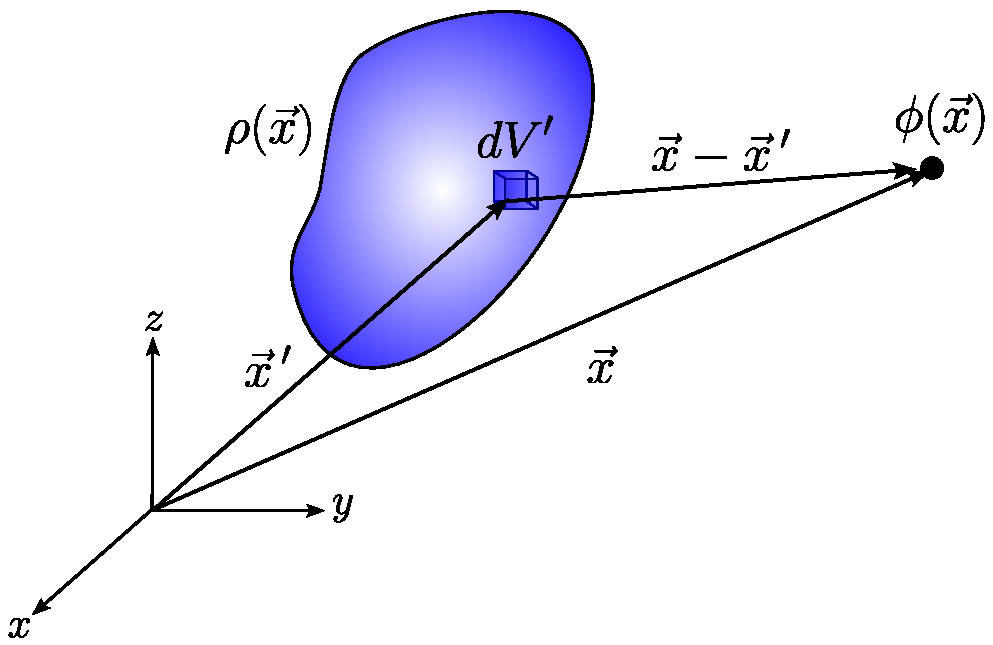
\includegraphics[width = 8cm]{Figuras/Distribucion-Cargas.pdf}
    \caption{Distribución de carga de densidad $\rho(\Vec{x})$.}
    \label{fig:PotencialDistribucion}
\end{figure}

Matemáticamente, podemos entender la convolución $f * g$ como \emph{el grado de traslape} entre dos pulsos, $f(y)$ y $g(-y)$, cuando uno $g(-y)$ se encuentra desplazado en $x$ unidades. Esta idea se puede observar en la figura \ref{fig:IdeaConvolucion}.

\begin{figure}[htbp]
    \centering
    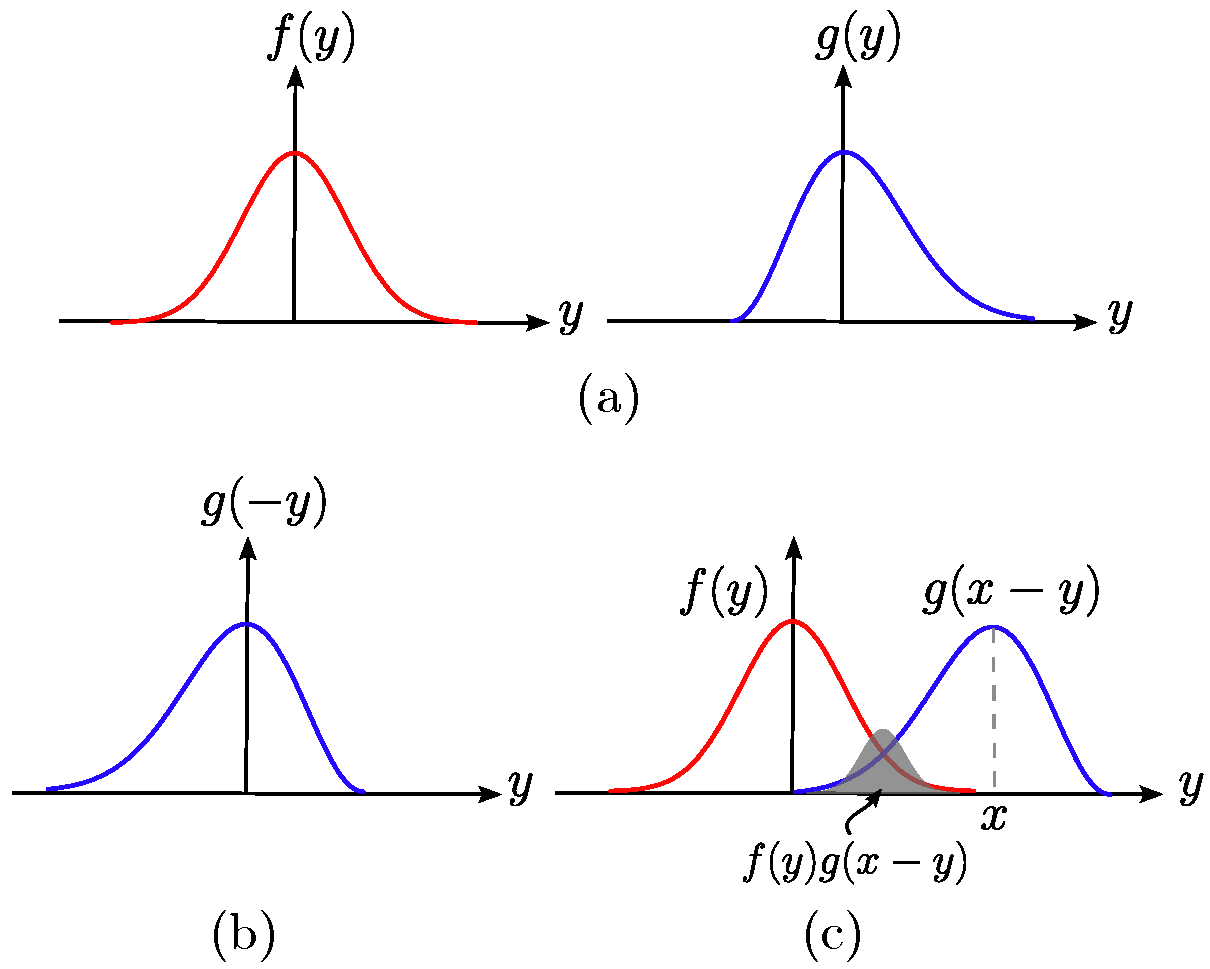
\includegraphics[width=10cm]{Figuras/Idea-Convolucion.pdf}
    \caption{Idea matemática de la convolución. En (a), se expresa cada función en términos de la variable de integración $y$. En (b), se refleja la gráfica de $g(y)$ con respecto al eje vertical, es decir, $g(y) \rightarrow g(-y)$. En (c), se traslada la gráfica de $g(-y)$, $x$ unidades. Luego, se traslapan las gráficas de $f(y)$ y $g(x-y)$ de tal forma que el área sombreada corresponde al valor de $f * g$ para ese valor de $x$.}
    \label{fig:IdeaConvolucion}
\end{figure}

% Entonces, $f * g$ mide el grado de traslape entre $f(y)$ y $g(-y)$, luego de trasladar $g$ a una distancia $x$.

\begin{propiedad}\textbf{Propiedades de la convolución.}

Sean $f(x)$, $g(x)$ y $h(x)$  funciones reales. Entonces, se verifican las siguientes propiedades:

\begin{enumerate}
    \item \textbf{Conmutatividad:}$$f(x) * g(x) = g(x) * f(x).$$
    
    \item \textbf{Asociatividad:} $$[f(x)*g(x)]*h(x) = f(x)*[g(x)*h(x)].$$
    
    \item \textbf{Distributividad:} $$f(x)*[g(x)+h(x)] = f(x)*g(x) + f(x)*h(x).$$ 
\end{enumerate}
\end{propiedad}

\newpage

\begin{teorema}[de convolución de Fourier]
Sean $f(x)$, $g(x)$ y $h(x)$  funciones reales y sean $\tilde{f}(k)$, $\tilde{g}(k)$ y $\tilde{h}(k)$ sus correspondientes transformadas de Fourier. 

\begin{itemize}
    \item Si $\tilde{h}(k) = \tilde{f}(k) \tilde{g}(k)$, entonces 
$$ h(x) = \frac{1}{\sqrt{2\pi}} (f * g)(x) = \frac{1}{\sqrt{2\pi}} \int_{-\infty}^{\infty} f(y) g(x-y) \,dy.$$ 

    \item Si $h(x) = f(x) g(x)$, entonces
    \begin{equation}
        \Tilde{h}(k) = \frac{1}{\sqrt{2\pi}}(\Tilde{f} * \Tilde{g})(k) = \frac{1}{\sqrt{2\pi}} \int_{-\infty}^{\infty} \Tilde{f}(y) \Tilde{g}(k-y) \,dy.
    \end{equation}
% $$$$
\end{itemize}
\end{teorema}

\begin{demo}
\ 

\begin{itemize}
    \item Supongamos que  $\tilde{h}(k) = \tilde{f}(k) \tilde{g}(k)$. Aplicando la transformada de Fourier inversa dada por \eqref{I.Fourier}, tenemos que 
\begin{align*}
   h(x) = \mathcal{F}^{-1} \{\tilde{h}(k)\} & = \mathcal{F}^{-1} \{\tilde{f}(k) \tilde{g}(k)\} \\
   & = \frac{1}{\sqrt{2\pi}} \int_{-\infty}^{\infty} \tilde{f}(k) \tilde{g}(k) e^{ikx} \,dk \\
   & = \frac{1}{\sqrt{2\pi}} \int_{-\infty}^{\infty}  \left( \frac{1}{\sqrt{2\pi}} \int_{-\infty}^{\infty} f(y) e^{-ik y} \,dy \right) \tilde{g}(k)  e^{ikx}  \,dk.
\end{align*}

Si el intercambio de orden de integración es posible, entonces 
\begin{align*}
  h(x) &= \frac{1}{\sqrt{2\pi}} \int_{-\infty}^{\infty}  f(y)  \left( \frac{1}{\sqrt{2\pi}} \int_{-\infty}^{\infty}  \tilde{g}(k)  e^{ikx} e^{-ik y}\,d k \right) \,dy \\
   & = \frac{1}{\sqrt{2\pi}} \int_{-\infty}^{\infty}  f(y)  \left( \frac{1}{\sqrt{2\pi}} \int_{-\infty}^{\infty}  \tilde{g}(k)  e^{ik(x-y)}\,d k \right) \,dy \\
   & = \frac{1}{\sqrt{2\pi}} \int_{-\infty}^{\infty}  f(y) g(x-y) \,dy = \frac{1}{\sqrt{2\pi}} (f * g)(x).
\end{align*}

Como la convolución es conmutativa:
$$h(x) = \frac{1}{2\pi} (f * g)(x) = \frac{1}{2\pi} (g * f)(x)  = \frac{1}{\sqrt{2\pi}} \int_{-\infty}^{\infty}  f(y) g(x-y) \,dy.$$

\item  Supongamos que $h(x) = f(x) g(x)$. Aplicando la transformada de Fourier dada por \eqref{T.Fourier}, tenemos que 
\begin{align*}
   \Tilde{h}(k) &=  \mathcal{F} \{f(x) g(x)\} \\
   &= \frac{1}{\sqrt{2\pi}} \int_{-\infty}^{\infty} f(x) g(x) e^{-ikx} \,dx \\
   &=  \frac{1}{\sqrt{2\pi}} \int_{-\infty}^{\infty} \left( \frac{1}{\sqrt{2\pi}} \int_{-\infty}^{\infty} \Tilde{f}(y) e^{iyx} \,dy \right) g(x) e^{-ikx} \,dx.
\end{align*}

Si el intercambio de orden de integración es posible, entonces 
\begin{align*}
   \Tilde{h}(k) &=  \frac{1}{\sqrt{2\pi}} \int_{-\infty}^{\infty} \Tilde{f}(y) \left( \frac{1}{\sqrt{2\pi}} \int_{-\infty}^{\infty} g(x) e^{iyx}  e^{-ikx}\,dx \right) \,dy \\
   &=  \frac{1}{\sqrt{2\pi}} \int_{-\infty}^{\infty} \Tilde{f}(y) \left( \frac{1}{\sqrt{2\pi}} \int_{-\infty}^{\infty} g(x) e^{-i(k-y)x} \,dx \right) \,dy \\
   &=  \frac{1}{\sqrt{2\pi}} \int_{-\infty}^{\infty} \Tilde{f}(y) \Tilde{g}(k-y) \,dy. 
\end{align*}

Por lo tanto,
$$\Tilde{h}(k) =  \frac{1}{\sqrt{2\pi}} (\Tilde{f} * \Tilde{g})(k) = \frac{1}{\sqrt{2\pi}} \int_{-\infty}^{\infty} \Tilde{f}(y) \Tilde{g}(k-y) \,dy.$$
\end{itemize}

\end{demo}


\begin{ejemplo}
    Sabiendo que \cite{Mauch}
    $$\mathcal{F}\left\{ \frac{2c}{x^2+c^2} \right\} = e^{-c|k|}, \quad \text{para} ~ c > 0.$$

    Podemos usar el teorema de convolución para encontrar la transformada de Fourier de
    \begin{equation}
      f(x) = \frac{1}{x^4+5x^2+4} = \frac{1}{(x^2+1)(x^2+4)}.    \label{EjConvo}
    \end{equation}
  
    En efecto,
    \begin{align*}
        \mathcal{F}\{f(x)\} &=  \mathcal{F}\left\{ \frac{1}{8} \frac{2}{x^2+1} \frac{4}{x^2+4} \right\} \\
        &= \frac{1}{8} \left( \int_{-\infty}^{\infty} e^{-|y|}e^{-2|k-y|} dy \right) \\
        &= \frac{1}{8} \left( \int_{-\infty}^0 e^{y}e^{-2|k-y|} dy +   \int_0^{\infty} e^{-y}e^{-2|k-y|} dy \right).
    \end{align*}

Si $k > 0$,
\begin{align*}
    \mathcal{F}\{f(x)\} &= \frac{1}{8} \left(  \int_{-\infty}^0 e^{y}e^{-2(k-y)} dy +  \int_0^k e^{-y}e^{-2(k-y)} dy + \int_k^{\infty} e^{-y}e^{2(k-y)} dy \right)  \\
    &= \frac{1}{8} \left(  \int_{-\infty}^0 e^{-2k+3y} dy +  \int_0^k e^{-2k+y} dy + \int_k^{+\infty} e^{2k-3y} dy \right) \\
    &= \frac{1}{8} \left( \frac{1}{3} e^{-2k} + e^{-k} - e^{-2k} + \frac{1}{3} e^{-k} \right) \\
    &= \frac{1}{6} e^{-k} - \frac{1}{12} e^{-2k}. 
\end{align*}

Si $k < 0$,
\begin{align*}
    \mathcal{F}\{f(x)\} &= \frac{1}{8} \left(  \int_{-\infty}^k e^{y}e^{-2(k-y)} dy +  \int_k^0 e^{y}e^{2(k-y)} dy + \int_0^{\infty} e^{-y}e^{2(k-y)} dy \right)  \\
    &= \frac{1}{8} \left(  \int_{-\infty}^k e^{-2k+3y} dy +  \int_k^0 e^{2k-y} dy + \int_0^{\infty} e^{2k-3y} dy \right) \\
    &= \frac{1}{8} \left( \frac{1}{3} e^{k} - e^{2k} + e^k + \frac{1}{3} e^{2k} \right) \\
    &= \frac{1}{6} e^{k} - \frac{1}{12} e^{2k}. 
\end{align*}

Por lo tanto, para $k$ positivo como negativo,
$$\boxed{\mathcal{F}\{f(x)\} =  \frac{1}{6} e^{-|k|} - \frac{1}{12} e^{-2|k|}} $$

Una mejor forma de encontrar la transformada de Fourier de \eqref{EjConvo} es, en primer lugar, descomponer la función en fracciones parciales,
$$f(x) = \frac{1}{3} \frac{1}{x^2+1} - \frac{1}{3} \frac{1}{x^2+4},$$

para luego hacer usar de la linealidad de la transformada.
\begin{align*}
     \mathcal{F}\{ f(x)\} &= \frac{1}{6} \mathcal{F} \left\{ \frac{2}{x^2+1}\right\} - \frac{1}{12} \mathcal{F} \left\{ \frac{4}{x^2+4} \right\}  \\
     &= \frac{1}{6} e^{-|k|} - \frac{1}{12} e^{-2|k|}.
\end{align*}

\end{ejemplo}

% \section{Aplicación de la transformada de Fourier}

% La transformada de Fourier es útil para resolver ecuaciones diferenciales en el dominio $(-\infty, \infty)$ con condiciones de borde homogéneas en el infinito. En particular, en ecuaciones diferenciales \underline{lineales} con \underline{coeficientes constantes}, debido a la propiedad de linealidad de la transformada.

% A continuación se ilustra el procedimiento a seguir mediante ejemplos.

% \begin{ejemplo}
%     Encuentre la solución general de la ecuación diferencial
%     $$y''(x) - y(x) = e^{-\alpha |x|}, \quad y(\pm \infty) = 0, \quad \alpha > 0, \alpha \neq 1.$$

%     \textbf{Solución:} La solución del caso homogéneo 
%     $$y''(x) - y(x) = 0,$$

%     está dada por
%     $$y_h(x) = c_1 e^{x} + c_2 e^{-x}, \quad c_1,c_2 \in \mathbb{R}.$$

%     Nos queda por encontrar la solución particular, para ello haremos uso de la transformada de Fourier. 

%     Primero, determinemos 
    
%     \begin{align*}
%         \mathcal{F}\left\{ e^{-\alpha |x|} \right\} &= \frac{1}{2\pi} \int_{-\infty}^{\infty} e^{-\alpha |x|} e^{-ikx} dx \\
%         &= \frac{1}{2\pi} \left(  \int_{-\infty}^{0} e^{x(\alpha -ikx)} dx +  \int_{0}^{\infty} e^{-x(\alpha + ik)} dx\right) \\
%         &= \frac{1}{2\pi} \left( \frac{1}{\alpha -ik} + \frac{1}{\alpha +ik} \right) \\
%         &= \frac{\alpha/\pi}{\alpha^2 + k^2}.
%     \end{align*}

%     Luego, apliquemos la transformada de Fourier a la ecuación diferencial:
%     \begin{align*}
%         \mathcal{F}\{ y''(x)\} - \mathcal{F}\{y(x)\ &=  \mathcal{F}\left\{ e^{-\alpha |x|} \right\} \\
%         \Rightarrow - k^2 \mathcal{F}\{y(x)\} - \mathcal{F}\{y(x)\} &= \frac{\alpha/\pi}{\alpha^2 + k^2}.
%     \end{align*}

%     Despejando la transformada de Fourier de la solución.
%     \begin{align*}
%         \mathcal{F}\{y(x)\} &= \frac{-\alpha/\pi}{(k^2 + \alpha^2)(k^2+1)} \\
%         &= - \frac{\alpha}{\pi} \frac{1}{\alpha^2-1} \left( \frac{1}{k^2+1} - \frac{1}{k^2+ \alpha^2}\right) \\
%         &= \frac{1}{\alpha^2-1} \left( \frac{\alpha/\pi}{k^2 + \alpha^2} - \alpha \frac{1/\pi}{k^2+1} \right.)
%     \end{align*}

%     Tomando la transformada inversa, obtenemos que
%     $$y(x) = \frac{e^{-\alpha|x| - \alpha e^{-|x|} }}{\alpha^2-1}.$$

%     Por lo tanto, la solución general es
%     $$\boxed{y(x) = \frac{e^{-\alpha|x| - \alpha e^{-|x|} }}{\alpha^2-1} + c_1 e^{x} + c_2 e^{-x}, \quad c_1,c_2 \in \mathbb{R}}$$
% \end{ejemplo}

% \begin{ejemplo}
%   Consideremos un oscilador armónico amortiguado sometido a una fuerza externa $g(t)$. La ecuación de movimiento del oscilador está dada por
% \begin{equation}
%  \ddot{x}(t) + 2 \alpha \dot{x}(t) + \omega_0^2 x(t) = f(t), \label{EDO-Oscilador}   
% \end{equation}

% donde $f(t) = g(t)/m$ y $\alpha$ es una constante asociada al amortiguamiento del sistema. En los primeros cursos de Ecuaciones Diferenciales Ordinarias (EDO) se trabaja con $f(t)$ sinusoidal, pero gracias a la transformada de Fourier, podemos extender este resultado para funciones $f(t)$ arbitrarias. 

% Aplicando la transformada de Fourier en la variable temporal, a saber,
% $$\mathcal{F}\{x(t)\} = \frac{1}{2\pi} \int_{-\infty}^{\infty} f(t) e^{-i\omega t} dt, $$

% a ambos lados de la ecuación diferencial \eqref{EDO-Oscilador}, obtenemos 
% \begin{align}
%     \mathcal{F}\left\{ \ddot{x}(t) + 2 \alpha \dot{x}(t) + \omega_0^2 x(t)\right\} &= \mathcal{F}\left\{ f(t)\right\} \nonumber\\
%     \Rightarrow   \mathcal{F}\left\{ \ddot{x}(t) \right\} + 2\alpha \mathcal{F}\left\{ \dot{x}(t) \right\} + \omega_0^2 \mathcal{F}\{x(t)\} &= \mathcal{F}\left\{ f(t)\right\}. \label{EDO-Transformada}
% \end{align}

% Si asumimos que 
% $$\lim_{x \to \pm \infty} x(t) = \lim_{x \to \pm \infty} \dot{x}(t) = 0,$$

% tenemos 
% \begin{align*}
%      \mathcal{F}\left\{ \ddot{x}(t) \right\} &= (i\omega)^2 \mathcal{F}\{x(t)\} = - \omega^2 \mathcal{F}\{x(t)\},\\
%       \mathcal{F}\left\{ \dot{x}(t) \right\} &= i \omega \mathcal{F}\{x(t)\}.
% \end{align*}

% Además, si definimos $F(\omega) := \mathcal{F}\left\{ f(t)\right\}$, la ecuación \eqref{EDO-Transformada} nos queda
% $$ - \omega^2 \mathcal{F}\{x(t)\} + 2 \alpha \omega i \mathcal{F}\{x(t)\} + \omega_0^2 \mathcal{F}\{x(t)\} = F(\omega).$$

% Despejando la transformada de Fourier de la solución:
% $$  \mathcal{F}\{x(t)\} = \frac{F(\omega)}{-\omega^2 - 2 \alpha i \omega + \omega_0^2}.$$

% Tomando la transformada inversa, obtenemos la solución 
% $$\boxed{x(t) = \int_{-\infty}^{\infty} \frac{F(\omega)}{(\omega_0^2-\omega^2) - 2 \alpha \omega i} e^{i\omega t} d\omega }$$  
% \end{ejemplo}


\section{Transformada de Laplace}

% \section{Definición}

\begin{defi}
Sea $f(t)$ una función a valores reales definida para $t \in [0, \infty[$. La \textbf{transformada de Laplace} de $f$ es la función $F$ definida mediante la integral impropia
$$F(s) := \int_0^{\infty} e^{-st} f(t) \,dt.$$

El dominio de $F(s)$ está formado por todos lo valores de $s$ (complejos) para los que la integral existe. Simbólicamente,
$$F(s) = \mathcal{L}\{f(t)\}.$$
\end{defi}

\begin{ejemplo}
Determine la transformada de Laplace de 
$$f(t) = e^{at}.$$

\textbf{Solución:} Por definición, 
\begin{align*}
    \mathcal{L}\{e^{at}\} = \int_0^{\infty} e^{-st} e^{at} \,dt &= \int_0^{\infty} e^{-(s-a)t} \,dt \\
    &= \left. - \frac{e^{-(s-a)t}}{s-a} \right|_0^{\infty} \\
    &= \frac{1}{s-a}, \quad \real(s) > a.
\end{align*}

En efecto, si hacemos $s = \real(s) + i \im(s)$, tenemos que
$$\lim_{t\to + \infty} \left| e^{-(s-a)t} \right| = \lim_{t\to + \infty} \left|e^{-(\real(s) - a)t} \right| = 0, \quad \real(s) > a. $$
\end{ejemplo}

\begin{ejemplo}
    Consideremos la transformada de Laplace de la \textbf{función de Heaviside},
    $$H(t-a) = \left\{ \begin{array}{cl}
     0,& \text{si} ~ t < a  \\
     1,& \text{si} ~ t > a
    \end{array} \right.,$$

    para un número real $a$ no negativo.
    \begin{align*}
        \mathcal{L}\{H(t-a)\} &= \int_0^{\infty} e^{-st} H(t-a) \,dt \\
        &= \int_a^{\infty} e^{-st} \,dt \\
        &= \left. - \frac{e^{-st}}{s}\right|_a^{\infty} \\
        &= \frac{e^{-as}}{s}, \quad \real(s) > 0.
    \end{align*}

    Ahora, consideremos $H(t-a)f(t-a)$.
    \begin{align*}
        \mathcal{L}\{H(t-a)f(t-a)\} &= \int_0^{\infty} e^{-st} H(t-a)f(t-a) \,dt \\
        &= \int_a^{\infty} e^{-st} f(t-a) \,dt \\
        &= \int_0^{\infty} e^{-s(t+a)} f(t) \,dt \\
        &= e^{-as} F(s).
    \end{align*}

\end{ejemplo}

\begin{ejemplo}
    Queda como ejercicio para el lector demostrar que
    \begin{align*}
        \mathcal{L}\{\cos(at)\} &= \frac{s}{s^2+a^2}, \quad \real(s) > 0, \\
        \mathcal{L}\{\sin(at)\} &= \frac{a}{s^2+a^2}, \quad \real(s) > 0.
    \end{align*}
\end{ejemplo}

En la mayoría de los casos será posible calcular $\mathcal{L}\{f(t)\}$ por evaluación directa. Sin embargo, no satisface la necesidad de determinar un conjunto razonable de condiciones que nos asegure la existencia de la transformada de Laplace de una función dada $f$.

A partir de la definición, es claro que $f$ debe escogerse de manera que
\begin{equation}
\int_0^{t_0} e^{-st} f(t) dt \label{Laplace1}
\end{equation}

exista para todo $t_0 > 0$. Ésto se logra exigiendo que $f$ sea seccionalmente continua en todo el intervalo $[0,t_0]$, con $t_0>0$. No obstante, no es suficiente para garantizar la existencia de $\mathcal{L}\{f(t)\}$ ya que al tomar el límite $t_0 \to \infty$ de \eqref{Laplace1}, ésta debe converger. A grandes rasgos, mostraremos que la transformada de Laplace de una función continua por partes existe, siempre que la función no crezca más rápido que una exponencial.

\begin{defi}
    Una función $f(t)$ es de \textbf{orden exponencial $\alpha$} en $[0,\infty[$ si existen constantes positivas $T$ y $M$ tales que
    $$\forall t \in [T, \infty[: ~ |f(t)| \leq M e^{\alpha t}.$$
\end{defi}

\begin{ejemplo}
\ 

    \begin{itemize}
        \item Toda función acotada es de orden exponencial 0.

        \item $t e^{2t}$ es de orden exponencial $\alpha$ para cualquier $\alpha > 2$. En efecto,
        $$\lim_{t \to \infty} \frac{t e^{2t}}{e^{\alpha t}} = \lim_{t \to \infty} \frac{t}{e^{(\alpha-2) t}} \overset{L'H}{=} \lim_{t \to \infty} \frac{1}{(\alpha -2 )e^{(\alpha-2) t}} = 0,$$

        para $\alpha > 2$. Eligiendo $M = 1$, por definición de límite, existe $T > 0$ tal que 
        $$\left|\frac{t e^{2t}}{e^{\alpha t}} \right| < 1 \Rightarrow |te^{2t}| < e^{\alpha t}, \quad \text{si} ~ t \geq T.$$
        
        \item $e^{t^2}$ no es de orden exponencial. En efecto,
        $$\lim_{t \to  \infty} \frac{e^{t^2}}{e^{\alpha t}} = \lim_{t \to \infty} e^{t(t-\alpha)} = \infty, \quad \mbox{para todo} ~ \alpha.$$

        Ésto es,
        $$(\forall M >0)(\exists T >0)\left(t \geq T \Rightarrow e^{t^2} > M e^{\alpha t}\right).$$

        \item $t^n, n \in \mathbb{N}$ es de orden exponencial $\alpha$ para cualquier $\alpha > 0$ (ejercicio para el lector).
    \end{itemize}
\end{ejemplo}

\begin{teorema}[de existencia] \label{ExistenciaLaplace}
Si $f$ es una función seccionalmente continua y de orden exponencial $\alpha$, entonces la transformada de Laplace
$$\mathcal{L}\{f(t)\} = \int_0^{\infty} e^{-st} f(t) \,dt$$

converge para $\real(s) > \alpha$. Más aún, la integral es absolutamente y uniformemente convergente para $\real(s) \geq \alpha_1 >  \alpha$.
\end{teorema}

\textbf{Observación:} Existen funciones que tienen transformada de Laplace y que no satisfacen las hipótesis del teorema. Por ejemplo, $f(t) = \frac{1}{\sqrt{t}}$ no es de orden exponencial, pues tiende a $\infty$ cuando $t \to 0^+$. Sin embargo,
\begin{equation*}
\mathcal{L}\{f(t)\} = \sqrt{\frac{\pi}{s}}.
\end{equation*}

En efecto, haciendo $x^2 = st$ y considerando que $\int_0^{\infty} e^{-x^2} dx = \frac{\sqrt{\pi}}{2}$, se tiene que
\begin{equation*}
\mathcal{L}\{t^{-1/2}\} = \int_0^{\infty} e^{-st}t^{-1/2}dt = \frac{2}{\sqrt{s}} \int_0^{\infty} e^{-x^2} dx = \sqrt{\frac{\pi}{s}}.
\end{equation*}

\begin{teorema}
    Bajo las mismas condiciones del teorema \ref{ExistenciaLaplace}, la transformada de Laplace $F(s)$ es holomorfa (analítica) en $\real(s) \geq \alpha_1 > \alpha$, es decir, la derivada $F'(s)$ existe en dicho semiplano.
\end{teorema}

En general, existe
\begin{shaded}
$$\frac{d^n}{ds^n} F(s) = (-1)^n \mathcal{L}\{t^n f(t)\}.$$
\end{shaded}

\begin{propo} \label{T.LaplaceLim}
Bajo las mismas condiciones del teorema \ref{ExistenciaLaplace},
$$\lim_{\real(s) \to \infty} F(s) = 0.$$
\end{propo}

\begin{demo}
    Si $f$ es de orden exponencial $\alpha$, entonces existen constantes  $T, M >0$ tales que
\begin{equation*}
|f(t)| \leq M e^{\alpha t}, \quad \forall t \geq T.
\end{equation*}

Luego,
\begin{eqnarray*}
\left|F(s)\right| = \left| \int_0^{+\infty} e^{-st} f(t) dt \right| &\leq &\left| \int_0^{T} e^{-st} f(t) dt \right| + \left| \int_T^{+\infty} e^{-st} f(t) dt \right| \\
& \leq & \int_0^T e^{-\real(s)t} |f(t)| dt +  \int_T^{+\infty} e^{-\real(s)t} |f(t)| dt \\
& \leq & I + \frac{M e^{-(\real(s)-\alpha)T}}{\real(s)-\alpha}, \quad \real(s) > \alpha
\end{eqnarray*}

donde $I = \int_0^T e^{-\real(s)t} |f(t)| dt$.

Como 
\begin{equation*}
\lim_{\real(s) \to +\infty} \left[ I + \frac{M e^{-(\real(s)-\alpha)T}}{\real(s) -\alpha} \right] = \cancelto{0}{\lim_{\real(s) \to +\infty} I} +  \cancelto{0}{\lim_{\real(s) \to +\infty} \frac{M e^{-(\real(s)-\alpha)T}}{\real(s) -\alpha}} = 0,
\end{equation*}

concluimos que
$$\lim_{s \to + \infty} F(s) = 0.$$
\end{demo}

\textbf{Observaciones:}

\begin{itemize}
\item[(a)] El contrarrecíproco del teorema es: si $\lim\limits_{s \to + \infty} \mathcal{L}\{f(t)\} \neq 0$, entonces no existe $f(t)$ tal que $F = \mathcal{L}\{f(t)\}$.

\item[(b)] Por observación $(a)$ podemos decir inmediatamente que funciones tales como $\frac{s+4}{s-1}, s, s^2, \sin(s)$, etc. no tienen transformada inversa de Laplace.
\end{itemize} 

\subsection{Transformada inversa de Laplace}

\begin{defi}
Dada una función $F(s)$, si existe una función $f(t)$ que sea continua en $[0, + \infty[$ y satisfaga
\begin{equation}
\mathcal{L}\{f(t)\} = F, \label{LaplaceInversa}
\end{equation}

entonces decimos que $f(t)$ es la \textbf{transformada inversa de Laplace} de $F(s)$ y utilizamos la notación $f = \mathcal{L}^{-1} \{F(s)\}$.
\end{defi}

Es natural preguntarse si la transformada inversa de Laplace es única, para ello basta con determinar si $\mathcal{L}$ es una aplicación inyectiva o no. El siguiente teorema (sin demostración) garantiza la inyectividad sin considerar los puntos de discontinuidad de las funciones.

\begin{teorema}[de Lerch]
 Sea $f$ y $g$ funciones continuas por tramos y de orden exponencial, y supongamos que existe un número real $s_0$ tal que
\begin{equation*}
\mathcal{L}\{f\}(s) = \mathcal{L}\{g\}(s), \quad \forall Re(s) >s_0.
\end{equation*}

Entonces, con la posible excepción de los puntos de discontinuidad, $f(t) = g(t)$ para todo $t >0$.
\end{teorema}

Por lo tanto, dos funciones continuas por tramos que satisfagan \eqref{LaplaceInversa}, sólo pueden diferir en sus puntos de discontinuidad. Luego, la completa unicidad se alcanza si se impone la continuidad a $f$.

Otra interrogante es: ¿es $\mathcal{L}$ un operador sobreyectivo?. La respuesta es no y viene avalada por el teorema \ref{T.LaplaceLim}.

La transformada inversa de Laplace puede ser calculada con la siguiente integral compleja conocida como la \textbf{fórmula de inversión de Mellin} o \textbf{integral de Bromwich} \cite{Arfken}.
\begin{shaded}
   $$ f(t) = \frac{1}{2\pi i} \int_{\gamma - i \infty}^{\gamma + i \infty} e^{st} F(s) \,ds,$$
\end{shaded}

donde $\gamma$ es una constante real que se encuentra a la derecha de las singularidades de $F(s)$.

\textbf{Observación:} Matemáticamente hablando, se debería escribir $$f(t) = \frac{1}{2\pi i} V.P. \int_{\gamma - i \infty}^{\gamma + i \infty} e^{st} F(s) \,ds,$$ 

pues 
$$f(t) = \frac{1}{2\pi i} \lim_{R \to \infty} \int_{L_R} e^{st} F(s) \,ds,$$ 

con $L_R: s = \gamma + it, - R\leq t \leq R$.

% \subsection*{Origen de la fórmula de inversión de Mellin*}

% Supondremos que $f(t)$ es de orden exponencial $\gamma$, entonces existen $T,M > 0$ tales que
% $$|f(t)| \leq M e^{\gamma t}, \quad \forall t \geq T,$$

% donde el número real $\gamma$ se escoge tal que la recta $x = \gamma$ esté a la derecha de todas las singularidades de $F(s)$.

% Por definición de la transformada de Laplace, se tiene que
% $$F(s) = \int_0^{\infty} e^{-su} f(u) \,du.$$

% Luego,
% $$\lim_{R \to \infty} \frac{1}{2\pi i} \int_{\gamma -i R}^{\gamma + i R} e^{st} F(s) \,ds = \lim_{R \to \infty} \frac{1}{2\pi i} \int_{\gamma -i R}^{\gamma + i R} \int_0^{\infty} e^{st-su} f(u) \,du \,ds.$$

% Evaluando la integral compleja, ésto es, $s = \gamma +i y$ y $ds = i dy$, con $- R\leq y \leq R$, obtenemos que
% \begin{align*}
%    \lim_{R \to \infty} \frac{1}{2\pi i} \int_{\gamma -i R}^{\gamma + i R} e^{st} F(s) \,ds &=  \lim_{R \to \infty} \frac{1}{2\pi i} \int_{- R}^{R} \int_0^{\infty} i e^{(\gamma + iy)t - (\gamma + i y)u} f(u) \,du \,dy \\
%    &= \lim_{R \to \infty} \frac{1}{2\pi} e^{\gamma t} \int_{- R}^{R} \int_0^{\infty} e^{i y t} e^{-\gamma u} e^{-iy u} f(u) \,du \,dy.
% \end{align*}

% Notemos que para $u \geq T$,
% $$| e^{i y t} e^{-\gamma u} e^{-iy u} f(u)| \leq e^{-\gamma u} |f(u)|.$$

% Por el teorema \ref{ExistenciaLaplace}, la integral de la transformada de Laplace $F(s)$ converge absolutamente, en específico para $s = \gamma$, luego
% $$\int_0^{\infty} |e^{-\gamma u} f(u)| \,du = \int_0^{\infty} e^{-\gamma u} |f(u)| \,du,$$

% converge. Así, usando el test de convergencia uniforme para integrales, la integral 
% $$\int_0^{\infty} e^{i y t} e^{-\gamma u} e^{-iy u} f(u) \,du $$

% converge uniformemente para $-R \leq y \leq R$. Luego, podemos intercambiar el orden de integración de acuerdo al teorema \ref{TeoA:OrdenIntegracion1} como sigue.
% \begin{align*}
%    \lim_{R \to \infty} \frac{1}{2\pi i} \int_{\gamma -i R}^{\gamma + i R} e^{st} F(s) \,ds &= \lim_{R \to \infty} \frac{1}{2\pi} e^{\gamma t} \int_{0}^{\infty} e^{-i y u} e^{-\gamma u} f(u) \left( \int_{-R}^R e^{i y t} dy \right) du \\
%    &=  \lim_{R \to \infty} \frac{1}{2\pi} e^{\gamma t}  \int_{-R}^R e^{iy t} dy  \int_{0}^{\infty} e^{-i y u} e^{-\gamma u} f(u) du \\
%    &= \frac{1}{2\pi} e^{\gamma t}  \int_{-\infty}^{\infty} e^{iyt} dy  \int_{0}^{\infty} e^{-i y u} [e^{-\gamma u} f(u)] du.
% \end{align*}

% Comparando con la ecuación \eqref{IntegralFourier}, podemos notar que 
% $$\int_{-\infty}^{\infty} e^{iy t} dy  \int_{0}^{\infty} e^{-i y u} [e^{-\gamma u} f(u)] du = \left\{ \begin{array}{cl}
%      2\pi e^{- \gamma t} f(t),& t > 0  \\
%      0,& t < 0
% \end{array} \right..$$

% Por lo tanto,
% $$  \lim_{R \to \infty} \frac{1}{2\pi i} \int_{\gamma -i R}^{\gamma + i R} e^{st} F(s) \,ds = f(t), \quad t > 0.$$

\subsection{\texorpdfstring{$F(s)$}{TEXT} con polos}

\begin{teorema}
    Si $F(s)$ es analítica excepto por las singularidades aisladas en $s_1, s_2, \dots, s_n$ y 
    $$\lim_{R \to \infty} \sup_{ |s - \gamma| = R} |F(s)| =  0.$$
   
   Entonces, la transformada de Laplace inversa de $F(s)$ es
    $$f(t) = \mathcal{L}^{-1}\{F(s)\} = \sum_{k= 1}^n Res(e^{st} F(s), s_k), \quad t > 0.$$
\end{teorema}

\begin{ejemplo}
    Determine la transformada inversa de Laplace de 
    $$F(s) = \frac{s^2}{s^4-1}.$$

    \textbf{Solución:} La transformada inversa de $F(s)$ está dada por la suma de los residuos de
    $$\psi(s) = e^{st} F(s) = e^{st} \frac{s^2}{(s-1)(s+1)(s-i)(s+i)}.$$

    Las singularidades de $\psi$ son $s = \pm 1, \pm i$, todos polos de orden 1. De esta manera, los residuos están dados por:
    \begin{align*}
        Res(\psi, 1) &= \lim_{s \to 1} (s-1) \psi(s) = \lim_{s\to 1} \left[e^{st} \frac{s^2}{(s+1)(s-i)(s+i)} \right] = \frac{e^t}{4},\\
        Res(\psi, -1) &= \lim_{s \to -1} (s+1) \psi(s) = \lim_{s\to -1} \left[e^{st} \frac{s^2}{(s-1)(s-i)(s+i)} \right] = -\frac{e^{-t}}{4}, \\
        Res(\psi, i) &= \lim_{s \to i} (s-i) \psi(s) = \lim_{s\to i} \left[e^{st} \frac{s^2}{(s-1)(s+1)(s+i)} \right] = \frac{e^{it}}{4i}, \\
        Res(\psi, -i) &= \lim_{s \to -i} (s+i) \psi(s) = \lim_{s\to -i} \left[e^{st} \frac{s^2}{(s-1)(s+1)(s-i)} \right] = -\frac{e^{-it}}{4i}.
    \end{align*}

    Por lo tanto,
    \begin{align*}
        \mathcal{L}^{-1} \left\{\frac{s^2}{s^4-1} \right\} &= Res(\psi,1) + Res(\psi,-1) + Res(\psi,i) + Res(\psi, -i) \\
        &= \frac{e^t}{4} - \frac{e^{-t}}{4} + \frac{e^{it}}{4i} - \frac{e^{-it}}{4i} \\
        &= \frac{1}{2} \frac{e^t - e^{-t}}{2} + \frac{1}{2} \frac{e^{it} - e^{-it}}{2i} \\
        &= \frac{1}{2} \sinh(t) + \frac{1}{2} \sin(t).
    \end{align*}
\end{ejemplo}

% \subsection{\texorpdfstring{$F(s)$}{TEXT} con puntos de ramificación*}

% Analizaremos este caso con un ejemplo.

% \begin{ejemplo} \label{Inv_Laplace_ej_branch}
%     Consideremos la transformada inversa de Laplace de
%     $$F(s) = \frac{1}{\sqrt{s}},$$

%     donde $\sqrt{s}$ es la rama principal de $s^{1/2}$. Así, la función tiene un corte de rama desde $s = 0$ a $s = - \infty$ y
%     $$\frac{1}{\sqrt{s}} = \frac{e^{-i \theta/2}}{\sqrt{r}}, \quad - \pi < \theta < \pi.$$

%     Sea $\gamma$ cualquier número positivo. La transformada inversa es
%     $$\mathcal{L}\left\{ \frac{1}{\sqrt{s}} \right\} = \frac{1}{2\pi i} \int_{\gamma - i\infty}^{\gamma + i \infty} e^{st} \frac{1}{\sqrt{s}} \,ds.$$

%     Para calcular la integral, primero consideremos el contorno representado en la figura \ref{fig:InvLaplaceBranchCut}. $C_2$ y $C_6$  son arcos de circunferencias centradas en el origen de radio $R$. $C_1$, $C_7$ y $C_8$ son segmentos que unen los dos arcos. $C_4$ es la semicircunferencia centrada en el origen en el lado derecho del eje imaginario de radio $\varepsilon < R$. Por último, $C_3$ y $C_5$ son lineas que unen los arcos circulares que van desde $-R + i\varepsilon$ a $i \varepsilon$ y $-i \varepsilon$ a $-R - i \varepsilon$, respectivamente.

%     \begin{figure}[H]
%         \centering
%         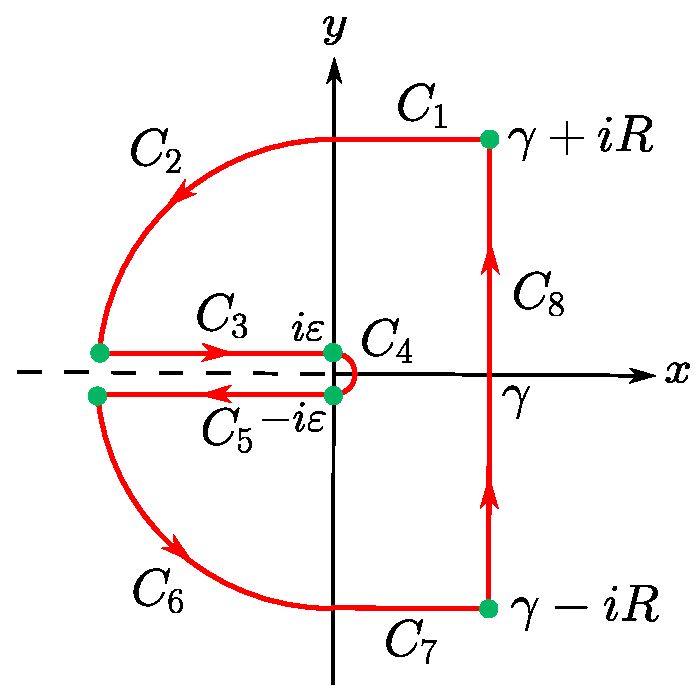
\includegraphics[scale = 0.6]{Figuras/InversaLaplace2.pdf}
%         \caption{Contorno de integración para la transformada inversa de Laplace $1/\sqrt{s}$.}
%         \label{fig:InvLaplaceBranchCut}
%     \end{figure}

%     Como el integrando es analítico en el interior del contorno cerrado, por el teorema de Cauchy-Goursat,
%     $$\sum_{k=1}^{8} \int_{C_k} e^{st} \frac{1}{\sqrt{s}} \,ds = 0.$$

%     Mostremos que la integral en torno a $C_1: s = x + i R, 0\leq x \leq \gamma$, se desvanece cuando $R \to \infty$. 

%     Para $s \in C_1$, tenemos que
%     $$\left|e^{st} \frac{1}{\sqrt{s}} \right| = \frac{e^{\real(s) t}}{\sqrt{|s|}} \leq \frac{e^{\gamma t}}{\sqrt{R}}.$$

%     Luego,
%     $$\left|\int_{C_1} e^{st} \frac{1}{\sqrt{s}} \,ds \right| \leq \int_0^{\gamma} \frac{e^{\gamma t}}{\sqrt{R}} \,dx = \frac{\gamma e^{\gamma t}}{\sqrt{R}} \overset{R \to \infty}{\longrightarrow} 0.$$

%     Similarmente, se prueba que la integral en torno a $C_7: s = x - i R, 0 \leq x \leq \gamma$, se desvanece cuando $R \to \infty$.

%     Ahora, mostremos que la integral en torno a $C_2: s = Re^{i\theta}, \pi/2 \leq \theta < \pi$, se desvanece cuando $R \to \infty$. 

%      Para $s \in C_2$, tenemos que
%     $$\left|e^{st} \frac{1}{\sqrt{s}} \right| = \frac{e^{\real(s) t}}{\sqrt{|s|}} = e^{R t \cos \theta }\frac{1}{\sqrt{R}}.$$

%     Luego,
%     $$\left|\int_{C_2} e^{st} \frac{1}{\sqrt{s}} \,ds \right| \leq \frac{1}{\sqrt{R}} \int_{\pi/2}^{\pi} e^{Rt \cos \theta} d\theta.$$

%     Haciendo la sustitución $\phi = \theta - (\pi/2) \Rightarrow d\phi = d\theta$, en la integral y usando la desigualdad de Jordan, obtenemos
%     $$\left|\int_{C_2} e^{st} \frac{1}{\sqrt{s}} \,ds \right| \leq \frac{1}{\sqrt{R}} \int_{0}^{\pi/2} e^{-Rt \sin \phi} d\phi \leq \frac{1}{\sqrt{R}} \frac{\pi}{2 R t}\overset{R \to \infty}{\longrightarrow} 0.$$

%     Similarmente, se prueba que la integral en torno a $C_6$ se desvanece.

%     Podemos mostrar que la integral en torno a $C_4: s = \varepsilon e^{i\theta}, -\pi/2 \leq \theta \leq \pi/2$, se desvanece cuando $\varepsilon \to 0$.

%     Para $s \in C_4$, tenemos que
%     $$\left|e^{st} \frac{1}{\sqrt{s}} \right| = \frac{e^{\real(s) t}}{\sqrt{|s|}} = \frac{e^{\varepsilon t \cos\theta}}{\sqrt{\varepsilon}} \leq  \frac{e^{\varepsilon t}}{\sqrt{\varepsilon}}.$$

%     Luego,
%     $$\left|\int_{C_4} e^{st} \frac{1}{\sqrt{s}} \,ds \right| \leq \frac{e^{\varepsilon t}}{\sqrt{\varepsilon}} \int_{-\pi/2}^{ \pi/2} \varepsilon d\theta = \frac{e^{\varepsilon t}}{\sqrt{\varepsilon}} (\pi \varepsilon) \overset{\varepsilon \to 0}{\longrightarrow} 0.$$

%     Entonces,
%     $$\int_{C_3} e^{st} \frac{1}{\sqrt{s}} \,ds + \int_{C_5} e^{st} \frac{1}{\sqrt{s}} \,ds + \int_{C_8} e^{st} \frac{1}{\sqrt{s}} \,ds = 0.$$

%     Tomando el límite $R \to \infty$ y $\varepsilon \to 0$, podemos expresar la transformada inversa de Laplace como
%     $$\mathcal{L}^{-1}\left\{ \frac{1}{\sqrt{s}}\right\} = \frac{1}{2\pi i} \int_{\gamma - i\infty}^{\gamma + i \infty} e^{st} \frac{1}{\sqrt{s}} \,ds = - \frac{1}{2\pi i} \lim_{R\to\infty}  \lim_{\varepsilon \to 0} \left[ \int_{C_3} e^{st} \frac{1}{\sqrt{s}} \,ds +  \int_{C_5} e^{st} \frac{1}{\sqrt{s}} \,ds\right].$$

%     Bajo estos límites, tenemos que en $C_3$, $s = x$, $ds = dx$, con $x$ desde $-\infty$ a $0$, y en $C_5$, $s = x$, $ds = dx$, con $x$ desde $0$ a $-\infty$.  Luego,
%     \begin{align*}
%        \mathcal{L}^{-1}\left\{ \frac{1}{\sqrt{s}}\right\} &= - \frac{1}{2\pi i} \int_{-\infty}^0 e^{xt} \frac{e^{-i\pi/2}}{\sqrt{-x}} \,dx - \frac{1}{2\pi i} \int_0^{-\infty} e^{xt} \frac{e^{i\pi/2}}{\sqrt{-x}} \,dx \\
%        &= -\frac{1}{2\pi} \int_{\infty}^0 e^{-xt} \frac{1}{\sqrt{x}} \,dx + \frac{1}{2\pi} \int_0^{\infty} e^{-xt} \frac{1}{\sqrt{x}} \,dx \\
%        &= \frac{1}{\pi} \int_0^{\infty} e^{-xt} \frac{1}{\sqrt{x}} \,dx.
%     \end{align*}

%     Haciendo la sustitución $u = xt \Rightarrow du = t dx$,
%     $$ \mathcal{L}^{-1}\left\{ \frac{1}{\sqrt{s}}\right\}  = \frac{1}{\pi \sqrt{t}} \int_0^{\infty} e^{-u} \frac{1}{\sqrt{u}} \,du.$$

%     Pero,
%     $$\int_0^{\infty} e^{-u} \frac{1}{\sqrt{u}} \,du = \Gamma\left( \frac{1}{2}\right) = \sqrt{\pi}.$$

%     Por lo tanto,
%     $$ \mathcal{L}^{-1}\left\{ \frac{1}{\sqrt{s}}\right\} = \frac{1}{\sqrt{\pi t}}, \quad t > 0.$$
% \end{ejemplo}

\subsection{Propiedades de la transformada de Laplace}    

\begin{teorema}
    Si $f$ y $g$ son funciones cuyas transformadas de Laplace existen para $\real(s) > \alpha$ y sean $a, b \in \mathbb{R}$. Entonces, 
\begin{enumerate}
    \item \textbf{Linealidad:} Para $\real(s) > \alpha$,
    $$\mathcal{L}\{a f(t) + b g(t)\} = a \mathcal{L}\{f(t)\} + b \mathcal{L}\{g(t)\}.$$ 

    \item \textbf{Escalonamiento:} Para $\real(s) > \alpha \cdot \beta$,
    $$\mathcal{L}\{f(\beta t) \} = \frac{1}{\beta} F \left( \frac{s}{\beta}\right), \quad \beta > 0.$$ 
    
    \item \textbf{Desplazamiento en el plano $s$:} Para $\real(s) > \alpha + a$,
    $$\mathcal{L}\{e^{at} f(t)\} = F(s-a).$$
\end{enumerate}
\end{teorema}

\begin{ejemplo}
    Determine la transformada de Laplace de $e^{at} \sin(bt)$.

    \textbf{Solución:} En la primera sección, vimos que
    $$\mathcal{L}\{\sin(bt)\} = F(s) = \frac{b}{s^2+b^2}, \quad \real(s) > 0.$$

    Luego, por la propiedad de desplazamiento,
    $$\mathcal{L}\{e^{at} \sin(bt)\} = F(s-a) = \frac{b}{(s-a)^2+b^2}, \quad \real(s) > a.$$
\end{ejemplo}

\begin{teorema}[Propiedad de la derivada]
    Sea $f$ continua en $]0, + \infty [$ y $f'(t)$ continua por tramos en $[0, + \infty[$, ambas de orden exponencial $\alpha$. Entonces, para $\real(s) > \alpha$,
    $$\mathcal{L}\{f'(t)\} = s \mathcal{L}\{f(t)\} - f(0^+),$$

    donde $f(0^+) = \lim\limits_{t \to 0^+} f(t)$. 
\end{teorema}

En general, la transformada de Laplace de derivadas de orden superior están dadas por el siguiente teorema.

\begin{teorema}[Transformada de Laplace de derivadas de orden superior]
 Sean $f, f', \dots, f^{(n-1)}$ continuas para todo $t>0$ y sea $f^{(n)}$ continua por tramos en $[0,+\infty[$, con todas estas funciones de orden exponencial $\alpha$. Entonces, para $\real(s) > \alpha$,
$$\mathcal{L}\{f^{(n)}(t)\} = s^n \mathcal{L}\{f(t)\} - s^{n-1} f(0^+) - s^{n-2} f'(0^+) - \cdots - f^{(n-1)}(0^+). \label{LaplaceDerivada}$$

\end{teorema}

\begin{ejemplo}
Calcule 
$$\mathcal{L}\left\{\sin^2(at)\right\}.$$   

\textbf{Solución:} Sea $f(t) = \sin^2(at)$, entonces
$$f'(t) = 2a \sin(at) \cos(at) = a \sin(2at).$$

Como $f(0) = 0$ y $\frac{2a^2}{s^2+4a^2} = \mathcal{L}\{f'(t)\} = s \mathcal{L}\{f(t)\} - f(0)$, obtenemos
$$\mathcal{L}\left\{\sin^2(at)\right\} = \frac{2a^2}{s(s^2+4a^2)}, \quad \real(s) > 0.$$
\end{ejemplo}

Hemos determinando la transformada de Laplace de la derivada de una función $f$, es natural preguntarse sobre la transformada de una función definida por una integral:
$$g(t) = \int_0^t f(t') \,dt'.$$

\begin{teorema}
     Sea la función $f(t)$ continua por tramos y de orden exponencial $\alpha$. Entonces,
     $$\mathcal{L} \left\{ \int_0^t f(t') \,dt'\right\} = \frac{1}{s} \mathcal{L}\{f(t)\}, \quad \real(s) > \alpha.$$
\end{teorema}

\begin{demo}
Caso particular del teorema \ref{Teo:Convolucion} para 
$$(f * g)(t) = \int_0^t f(u) g(t-u) \,du,$$

con $g(t) = 1$.
\end{demo}

Para funciones periódicas, tenemos el siguiente teorema.

\begin{teorema}
 Sea $f$ una función continua por tramos en el intervalo $[0,T]$ y periódica con periodo $T>0$. Entonces $f$ tiene transformada de Laplace dada por
\begin{equation*}
\mathcal{L}\{f(t)\} = \frac{\int_0^T e^{-st} f(t) dt}{1-e^{-Ts}}, \quad \real(s) > 0.
\end{equation*}
   
\end{teorema}

\begin{ejemplo}
    Encuentre la transformada de Laplace de
    $$f(t) = \left\{ \begin{array}{cl}
     1,& \text{si} ~ 0 \leq t < \pi  \\
     0,& \text{si} ~ \pi \leq t < 2\pi
    \end{array} \right.$$

    y $f(t+ 2\pi) = f(t)$ para $t > 0$, ésto es, $f(t)$ es periódica para $t > 0$.

    \textbf{Solución:} Como $f$ es periódica de periodo $T = 2\pi$, tenemos que
    \begin{align*}
        \mathcal{L}\{f(t)\} &= \frac{\int_0^{2\pi} e^{-st} f(t) \,dt}{1-e^{-2\pi s}} \\
        &= \frac{\int_0^{\pi} e^{-st}\,dt}{1-e^{-2\pi s}} \\
        &= \frac{1-e^{-\pi s}}{s(1-e^{-2\pi s})} \\
        &= \frac{1}{s(1+e^{-\pi s})}.
    \end{align*}
\end{ejemplo}

\begin{teorema}[Integral de una transformada]
   Si $\int_0^{\beta} \frac{f(t)}{t} \,dt$ existe para $\beta > 0$ y $f(t)$ es de orden exponencial $\alpha$, entonces
   $$\mathcal{L}\left\{\frac{f(t)}{t}\right\} = \int_s^{\infty} F(u) \,du, \quad s > \alpha.$$
\end{teorema}

\subsection{Convolución}

\begin{defi}
   Sean $f$ y $g$ funciones continuas por tramos en $[0, \infty[$. La \textbf{convolución} de $f$ y $g$, que se denota $f*g$, se define como
\begin{equation*}
(f*g)(t) := \int_0^t f(t-u)g(u) \, du.
\end{equation*}  
\end{defi}

Es claro que la convolución es distinta de la multiplicación común. Por ejemplo, $1*1 = t \neq 1$, y en general, $1*f \neq f$. Sin embargo, la convolución sí satisface algunas propiedades de la multiplicación.

\begin{teorema}[Propiedades de la convolución]
Sean $f$, $g$ y $h$ continuas por tramos en $[0,  \infty[$. Entonces,

\begin{itemize}
\item[(i)] $f*g = g*f$,

\item[(ii)] $f*(g*h) = (f*g)*h$,  

\item[(iii)] $f*(g+h) = f*g + f*h$. 
\end{itemize} 
\end{teorema}

Al igual que para la transformada de Fourier, la transformada de Laplace de la convolución obedece el siguiente teorema.

\begin{teorema}[de Convolución] \label{Teo:Convolucion}
    Sean $f$ y $g$ funciones continuas por tramos, de orden exponencial, tales que:
    \begin{equation*}
    \mathcal{L}\{f(t)\} = F(s) ~~\mbox{y}~~ \mathcal{L}\{g(t)\} = G(s),
    \end{equation*}

    entonces
    \begin{equation*}
    \mathcal{L}\{(f*g)(t)\} = F(s)G(s),
    \end{equation*}

    o, de manera equivalente,
    \begin{equation*}
    \mathcal{L}^{-1}\{F(s)G(s)\}(t) = (f*g)(t).
    \end{equation*}    
\end{teorema}

\begin{demo}

Tomando la transformada de Laplace de la convolución $f * g$,
$$\mathcal{L}\{(f*g)(t)\} = \int_0^{\infty} e^{-st} \int_0^t f(t-u) g(u) \,du \,dt = \int_0^{\infty} \int_0^t e^{-st}  f(t-u) g(u) \,du \,dt.$$

La región de integración se ilustra en la figura \ref{fig:Convolucion2}.

\begin{figure}[H]
    \centering
    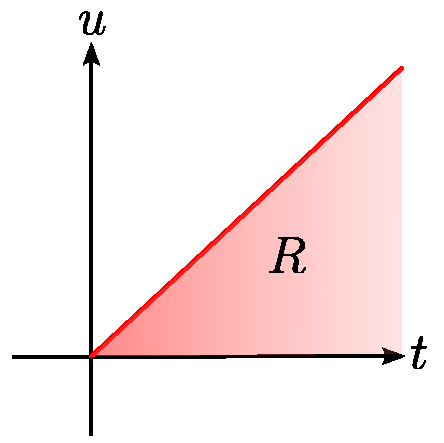
\includegraphics[scale = 0.6]{Figuras/Laplace-Convolucion-2.pdf}
    \caption{Región de integración.}
    \label{fig:Convolucion2}
\end{figure}

Luego, haciendo un cambio en el orden de integración, se tiene
$$\mathcal{L}\{(f*g)(t)\} = \int_0^{\infty} \int_u^{\infty} e^{-st} f(t-u) g(u) \,dt\,du.$$

Si hacemos el cambio de variable $v = t-u$ en la integral interior, obtenemos que
\begin{align*}
    \mathcal{L}\{(f*g)(t)\} &= \int_0^{\infty} g(u) \int_0^{\infty} e^{-s(u+v)} f(v) \,dv \,du \\
    &= \left(\int_0^{\infty} g(u) e^{-su} du \right)\left(\int_0^{\infty} f(v) e^{-sv} \,dv  \right) \\
    &= F(s)G(s). 
\end{align*}

\end{demo}

\begin{ejemplo}
Calcule
$$\mathcal{L}^{-1} \left\{ \frac{s}{(s^2+1)^2} \right\}.$$

\textbf{Solución:} Notemos que 
\begin{equation*}
\mathcal{L}^{-1} \left\{ \frac{s}{(s^2+1)^2} \right\} = \mathcal{L}^{-1} \left\{ \frac{s}{s^2+1} \cdot \frac{1}{s^2+1} \right\}.
\end{equation*}

Como
\begin{equation*}
\mathcal{L}\{\cos(t)\} = \frac{s}{s^2+1} ~~\mbox{y}~~ \mathcal{L}\{\sin(t)\} = \frac{1}{s^2+1},
\end{equation*}

tenemos, por el teorema de convolución, que
\begin{align*}
    \mathcal{L}^{-1} \left\{ \frac{s}{(s^2+1)^2} \right\} &=\cos(t) *\sin(t)  \\
    &= \int_0^t \sin(t-u) \cos(u) \,du \\
    &= \int_0^t (\sin(t) \cos(u) - \cos(u) \sin(u)) \cos(u) \,du  \\
    &= \sin(t) \int_0^t \cos^2(u) \,du - \cos(t) \int_0^t \sin (u) \cos(u) \,du \\
    &= \sin(t) \left[ \frac{1}{2} u + \frac{\sin(2u)}{4} \right]_0^t - \cos(t) \left[ \frac{\sin^2(u)}{2} \right]_0^t \\
    &= \frac{t \sin(t)}{2} + \frac{\sin(2t)}{4} \sin(t) - \cos(t) \frac{\sin^2(t)}{2} \\
    &= \frac{t \sin(t) }{2}.
\end{align*}

Por lo tanto,
$$\mathcal{L}^{-1} \left\{ \frac{s}{(s^2+1)^2} \right\} = \frac{t \sin(t) }{2}.$$   
\end{ejemplo}

\subsection{Aplicaciones de la transformada de Laplace}

La transformada de Laplace, al igual que la transformada de Fourier, nos permite convertir ecuaciones diferenciales en ecuaciones algebraicas, con una diferencia: se requiere el valor de la función en un punto dado. Lo anterior nos entrega una ligera ventaja y es que una vez que se invierta la transformada, tendremos de inmediato la solución al problema, recalcando que el dominio de validez de la función encontrada es para $t > 0$. Otra diferencia relevante es que, mientras la transformada de Fourier sólo se puede aplicar a funciones que decrecen rápidamente a cero, la transformada de Laplace está bien definida incluso para funciones de crecimiento exponencial. Entonces, si estamos en presencia de un sistema físico caracterizado por una variable que crece exponencialmente, es bastante probable que la transformada de Fourier dé resultados sin sentido físico.

A continuación expondremos dos situaciones en las cuales el uso de la transformada de Laplace es ventajoso.

\subsubsection{Ecuaciones diferenciales lineales con coeficientes constantes}

\begin{ejemplo}
    Consideremos la ecuación diferencial
    $$y'(t) + y(t) = \cos(t), \quad \text{para} ~ t > 0, \quad y(0) = 1.$$

    Apliquemos la transformada de Laplace a ambos lados de la ecuación:
    $$\mathcal{L}\{y'(t)\} - \mathcal{L}\{y(t)\} = \mathcal{L}\{\cos(t)\}.$$

    Evaluamos la transformada de la primera derivada, usando los teoremas enunciados durante el capítulo.
    $$\mathcal{L}\{y'(t)\} = s Y(s) - y(0) = s Y(s) - 1,$$

    donde $Y(s) = \mathcal{L}\{y(t)\}$. Luego, la ecuación diferencial nos queda:
    \begin{align*}
        sY(s) - 1 + Y(s) &= \frac{s}{s^2+1} \\
        \Rightarrow \quad Y(s) &= \frac{s}{(s+1)(s^2+1)} + \frac{1}{s+1} \\
        \Rightarrow \quad Y(s) &= \frac{1/2}{s+1} + \frac{1}{2} \frac{s+1}{s^2+1}.
    \end{align*}

    Aplicando la transformada de Laplace inversa,
    $$y(t) = \frac{1}{2} e^{-t} + \frac{1}{2} \cos(t) + \frac{1}{2} \sin(t), \quad t > 0.$$
\end{ejemplo}

% \subsubsection{Ecuaciones integrales}

% Una \textbf{ecuación integral} es aquella ecuación donde la función incógnita $\varphi(x)$ se encuentra dentro de una integral. Estas ecuaciones integrales se clasifican en dos formas \cite{Arfken}:
% \begin{itemize}
%     \item Si los límites de integración están fijos, llamamos la ecuación una \textbf{ecuación de Fredholm}; si un límite es variable, es una \textbf{ecuación de Volterra}.

%     \item Si la función incógnita aparece solo en la integral, la etiquetamos como de \textbf{primera especie}. Si aparece tanto dentro como fuera de la integral, la etiquetemos como de \textbf{segunda especie}.
% \end{itemize}

% A continuación algunos ejemplos de estas definiciones donde $\varphi(t)$ es la función desconocida, $K(x,t)$ una función de dos variables que la llamaremos \textbf{kernel}, y $f(x)$ una función que asumimos conocida.

% \begin{enumerate}
%     \item \textbf{Ecuación de Fredholm de primera especie}:
%     $$f(x) = \int_a^b K(x,t) \varphi(t) \,dt.$$

%     \item \textbf{Ecuación de Fredholm de segunda especie}:
%     $$\varphi(x) = f(x) + \lambda \int_a^b K(x,t) \varphi(t) \,dt.$$

%     \item \textbf{Ecuación de Volterra de primera especie}:
%     $$f(x) = \int_a^x K(x,t) \varphi(t) \,dt.$$

%     \item \textbf{Ecuación de Volterra de segunda especie}:
%     $$\varphi(x) = f(x) + \int_a^x K(x,t) \varphi(t) \,dt.$$
% \end{enumerate}

% En esta sección nos enfocaremos en ecuaciones de Volterra para $K(x,t) = K(x-t)$, de tal forma que
% $$\int_a^x K(x,t) \varphi(t) \,dt = (K * \varphi)(x).$$

% Para ilustrar el método, consideremos la situación física planteada en el siguiente ejemplo.

% \begin{ejemplo}[Problema de la tautócrona]
%     Una partícula de masa $m$ resbala (parte del reposo), sin roce, sobre una curva bajo el efecto de la gravedad. Buscamos determinar la forma de la curva de modo que el tiempo que le toma a la partícula en llegar al suelo sea independiente del punto de lanzamiento. 

%     \begin{figure}[H]
%         \centering
%         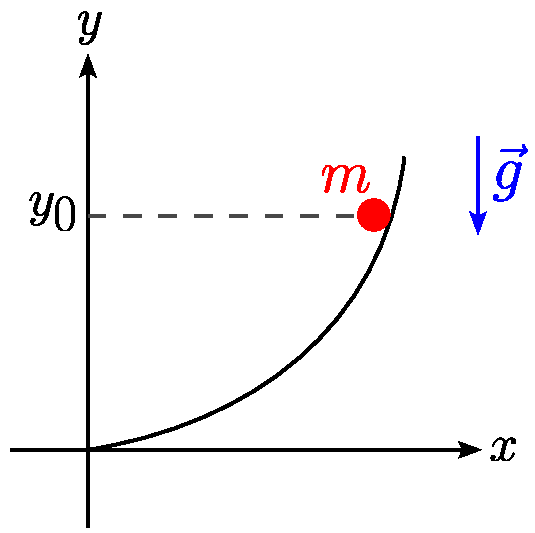
\includegraphics[scale = 0.65]{Figuras/tautocrona.pdf}
%         \caption{Esquema de la situación física.}
%         \label{fig:tautocrona}
%     \end{figure}

%     Como estamos en presencia de fuerzas conservativas, la  energía se conserva durante todo el trayecto para todo $y$, ésto es,
%     \begin{alignat*}{3}
%     &               &\quad   \text{Energía inicial en $y_0$} &= \text{Energía final en $y$} \\
%     &  \Rightarrow  &\quad      mgy_0 &= \frac{1}{2} mv^2 + mgy \\
%     &  \Rightarrow  &\quad   \frac{1}{2} mv^2 &= mg(y_0 - y) \\
%     &  \Rightarrow  &\quad   v &= \sqrt{2 g} \sqrt{y_0-y}, 
%     \end{alignat*}   
    
%     donde $y_0$ es la altura inicial. El tiempo de descenso está dado por
%     $$T(y_0) = \int \frac{ds}{v} = \int_{y_0}^0 \frac{1}{v} \frac{ds}{dy} dy = - \int_0^{y_0} f(y) (y_0 - y)^{-1/2} \frac{1}{\sqrt{2g}} dy,$$

%     donde $f(y) = ds/dy$. Ahora, si suponemos que $T(y_0)$ es constante $T_0$, ésto es, independiente del punto de partida $y_0$. La condición queda
%     $$\int_0^{y_0} f(y) (y_0 - y)^{-1/2} \,dy = C_0,$$

%     donde $C_0 = -\sqrt{2g} T_0$. Aplicando la transformada de Laplace  a ambos lados de la ecuación:
%     $$\mathcal{L}\left\{\int_0^{y_0} f(y) (y_0 - y)^{-1/2} \,dy \right\} = \mathcal{L}\{C_0\} = \frac{C_0}{s}.$$
    
%     Por el teorema de convolución, tenemos que
%     $$\mathcal{L}\{f(y)\} \mathcal{L}\{y^{-1/2}\} = \frac{C_0}{s} \Rightarrow \mathcal{L}\{f(y)\} = \frac{C_0/s}{\mathcal{L}\{y^{-1/2}\}}.$$

%     Pero,
%     $$\mathcal{L}\{y^{-1/2}\} = \int_0^{\infty} e^{-sy} \frac{1}{\sqrt{y}} \,dy \overset{\textcolor{blue}{t = sy}}{=} \frac{1}{\sqrt{s}}\int_0^{\infty} e^{-t} \frac{1}{\sqrt{t}} \,dt = \frac{\Gamma\left(\frac{1}{2}\right)}{\sqrt{s}}.$$

%     Así,
%     $$\mathcal{L}\{f(y)\} = \frac{C_0}{s} \frac{\sqrt{s}}{\Gamma\left(\frac{1}{2}\right)} = \frac{C_0}{\sqrt{\pi}} \frac{1}{\sqrt{s}}.$$

%     Tomando la transformada inversando y usando el resultado del ejemplo \ref{Inv_Laplace_ej_branch}, obtenemos 
%     $$f(y) = \frac{C_0}{\pi} \frac{1}{\sqrt{y}} = \frac{C}{\sqrt{y}},$$

%     donde $C = C_0/\pi$. Recordando que $f(y) = ds/dy$, notemos que
%     \begin{align*}
%         ds^2 = dx^2 + dy^2 &\Rightarrow dx = \sqrt{ds^2 - dy^2} \\
%         &\Rightarrow dx = \sqrt{\left( \frac{ds}{dy} dy\right)^2 - dy^2} \\
%         &\Rightarrow dx = \sqrt{\left(\frac{ds}{dy}\right)^2 - 1} \,dy \\
%         &\Rightarrow \frac{dx}{dy} = \sqrt{\frac{C^2}{y} - 1}. 
%     \end{align*}

%     Integrando con respecto a $y$,
%     $$x(y) = \int \sqrt{\frac{C^2}{y} - 1} \,dy.$$

%     Haciendo el cambio de variable $y = C^2 \sin^2 (\phi) \Rightarrow dy = 2 C^2 \sin(\phi) \cos(\phi) \,d\phi$,
%     \begin{align*}
%         x &= \int \sqrt{\csc^2(\phi) - 1} \, 2 C^2 \sin(\phi) \cos(\phi) \,d\phi \\
%         &= 2C^2 \int \sqrt{\cot^2(\phi)}  \sin(\phi) \cos(\phi) \,d\phi \\
%         &= 2C^2 \int \cos^2(\phi) \,d\phi \\
%         &=  \frac{C^2}{2} (2\phi + \sin(2\phi)) + D,
%     \end{align*}

%     donde $D$ es una constante de integración. Entonces,
%     \begin{align*}
%         x &= \frac{C^2}{2} (2\phi + \sin(2\phi)) + D, \\
%         y &= \frac{C^2}{2} (1 - \cos(2\phi)).
%     \end{align*}

%     La curva debe pasar por el origen $(0,0)$, así que $D = 0$, y si definimos un nuevo parámetro $\theta = 2\phi$, encontramos que
%     \begin{align*}
%         x &= \frac{C^2}{2} (\theta + \sin(\theta)), \\
%         y &= \frac{C^2}{2} (1 - \cos(\theta)).
%     \end{align*}

%     Estas son las ecuaciones paramétricas de un cicloide.
% \end{ejemplo}

\subsubsection{Sistema de ecuaciones lineales}

La transformada de Laplace puede ser usada para convertir un sistema de ecuaciones diferenciales con coeficientes constantes en un sistema de ecuaciones algebraicas. 

\begin{ejemplo}
    Consideremos el circuito de la figura \ref{fig:Circuit}. 
    
    \begin{figure}[H]
        \centering
        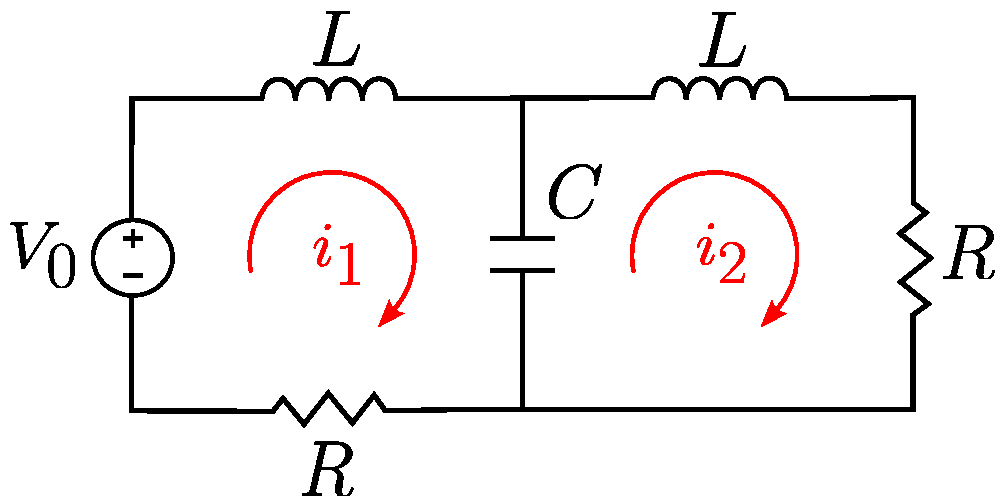
\includegraphics[scale = 0.65]{Figuras/Circuito.pdf}
        \caption{Circuito eléctrico.}
        \label{fig:Circuit}
    \end{figure}
    
    Usando las leyes de Kirchhoff, encontramos el siguiente sistema de ecuaciones diferenciales.
    \begin{align*}
        L \frac{di_1}{dt} + Ri_1 + \frac{q}{C} &= V_0, \\
        L \frac{di_2}{dt} + Ri_2 - \frac{q}{C} &= 0, \\
        \frac{dq}{dt} &= i_1 - i_2.
    \end{align*}
    
    Inicialmente el capacitador se encuentra descargado y las corrientes inducidas por las inductancias son despreciables de tal forma que se tienen las condiciones iniciales:
    $$i_1(0) = i_2(0) = \frac{V_0}{2R}, \quad q(0) = 0.$$

    Aplicamos la transformada de Laplace al sistema de ecuaciones diferenciales.
    \begin{align*}
        L\left( sI_1(s) - \frac{V_0}{2R} \right) + RI_1(s) + \frac{Q(s)}{C} &= \frac{V_0}{s}, \\
       L\left( sI_2(s) - \frac{V_0}{2R} \right) + RI_2(s) - \frac{Q(s)}{C}  &= 0, \\
        sQ(s) &= I_1(s) - I_2(s),
    \end{align*}

    donde $I_1(s) = \mathcal{L}\{i_1(t)\}$, $I_2(s) = \mathcal{L}\{i_2(t)\}$ y $Q(s) = \mathcal{L}\{q(t)\}$. Despejando estas cantidades:
    \begin{align*}
        I_1 &= \frac{V_0}{2} \left(\frac{1}{Rs} + \frac{1/L}{s^2 + R s/L + 2/(CL)} \right) \\
        I_2 &= \frac{V_0}{2} \left(\frac{1}{Rs} - \frac{1/L}{s^2 + R s/L + 2/(CL)} \right) \\
            Q &= \frac{C V_0}{2} \left( \frac{1}{s} - \frac{s+R/L}{s^2 + Rs/L + 2/(CL)} \right)
    \end{align*}

    Factorizando las polinomios de los denominadores.
    \begin{align*}
        I_1 &= \frac{V_0}{2} \left(\frac{1}{Rs} + \frac{1/L}{(s+\alpha - i \omega)(s + \alpha + i \omega)} \right) \\
        I_2 &= \frac{V_0}{2} \left(\frac{1}{Rs} - \frac{1/L}{(s+\alpha - i\omega)(s+\alpha + i \omega)} \right) \\
        Q &= \frac{C V_0}{2} \left( \frac{1}{s} - \frac{s+2\alpha}{(s+\alpha - i\omega)(s+\alpha + i \omega))} \right).
    \end{align*}

    Aquí hemos definido
    $$\alpha = \frac{R}{2L} \quad \text{y} \quad \omega^2 = \frac{2}{LC} - \alpha^2.$$

    Expandiendo las funciones en fracciones parciales.
    \begin{align*}
        I_1 &= \frac{V_0}{2} \left(\frac{1}{Rs} + \frac{i}{2\omega L} \left(\frac{1}{s+\alpha + i\omega} - \frac{1}{s+\alpha - i\omega} \right) \right) \\
        I_2 &= \frac{V_0}{2} \left(\frac{1}{Rs} - \frac{i}{2\omega L} \left(\frac{1}{s+\alpha + i\omega} - \frac{1}{s+\alpha - i\omega} \right) \right) \\
        Q &= \frac{C V_0}{2} \left( \frac{1}{s} + \frac{i}{2\omega} \left( \frac{\alpha + i\omega}{s+\alpha - i\omega} - \frac{\alpha - i \omega}{s+\alpha +i\Omega} \right) \right).
    \end{align*}

    Ahora, aplicamos la transformada inversa, teniendo en consideración que
    $$\mathcal{L}^{-1}\left\{ \frac{1}{s-a} \right\} = e^{at},$$
     \begin{align*}
        i_1 &= \frac{V_0}{2} \left(\frac{1}{R} + \frac{i}{2\omega L} \left( e^{(-\alpha - i\omega)t} - e^{(-\alpha + i\omega)t}\right) \right) \\
        i_2 &= \frac{V_0}{2} \left(\frac{1}{R} - \frac{i}{2\omega L} \left( e^{(-\alpha - i\omega)t} - e^{(-\alpha + i \omega)t}\right) \right) \\
        q &= \frac{C V_0}{2} \left( 1 + \frac{i}{2\omega} \left( (\alpha + i\omega) e^{(-\alpha + i \omega)t} - (\alpha - i\omega)e^{(-\alpha - i\omega)t} \right) \right).
    \end{align*}

    Simplicando las expresiones, obtenemos las soluciones.
    \begin{align*}
        i_1 &= \frac{V_0}{2} \left(\frac{1}{R} + \frac{1}{\omega L} e^{-\alpha t}\sin(\omega t) \right), \\
        i_2 &= \frac{V_0}{2} \left(\frac{1}{R} - \frac{1}{\omega L} e^{-\alpha t}\sin(\omega t) \right), \\
        q &= \frac{CV_0}{2} \left( 1- e^{-\alpha t} \left( \cos(\omega t) + \frac{\alpha}{\omega} \sin(\omega t) \right)\right).
    \end{align*}
\end{ejemplo}








 
